%%%%%%%%%%%%%%%%%%%%%%%%%%%%%%  IEEEsample.tex
%%%%%%%%%%%%%%%%%%%%%%%%%%%%%%%%%%%%%%%%%
%%%%%%%%%%%%%%%%%%%%%%%    More information: see the header of IEEEtran.sty
%%%%%%%%%%%%%%%%%%%%%%%
%%%%%%%%%%%%%%%%%%%%%%%%%%%%%%%%%%%%%%%%%%%%%%%%%%%%%%%%%%%%%%%%%%%%%%%%%%%%%%%%
%%%%

\documentclass[10pt,twoside, onecolumn]{IEEEtran}
%\documentclass[conference]{IEEEtran}

%%%\IEEEoverridecommandlockouts

\usepackage[ruled]{./algorithm2e}
%%for algorithm2e package, label has to be following caption in the same line!!!
\renewcommand{\algorithmcfname}{ALGORITHM}
\SetAlFnt{\small}
\SetAlCapFnt{\small}
\SetAlCapNameFnt{\small}
\SetAlCapHSkip{0pt}
\IncMargin{-\parindent}



%% \RequirePackage{times}
%% \RequirePackage{algorithmic}
%% \PassOptionsToPackage{boxed}{algorithm}
%% \RequirePackage{algorithm}
%% \RequirePackage{multicol}
%\renewcommand{\algorithmicrequire}{\textbf{Inputs:}}
%\renewcommand{\algorithmicensure}{\textbf{Outputs:}}
%\DeclareMathAlphabet{\mathtsl}{OT1}{ptm}{m}{sl}

%\def\BibTeX{{\rm B\kern-.05em{\sc i\kern-.025em b}\kern-.08em1
%    T\kern-.1667em\lower.7ex\hbox{E}\kern-.125emX}}

%\newtheorem{theorem}{Theorem}
%\newtheorem{lemma}{Lemma}
%\newtheorem{example}{Example}
%\newtheorem{corollary}{Corollary}

\RequirePackage{amssymb, mathptm}
\usepackage{amsbsy}
\usepackage{graphicx}
\usepackage{helvet}
\usepackage{enumerate}
\usepackage{amsmath}
\usepackage{amsfonts}
\usepackage{graphicx}
\usepackage{multirow}
\usepackage{subfig}
\usepackage{comment}



%%indent in algorithm


%\setcounter{page}{1}


% New command for the table notes.
\def\tabnote#1{{\small{#1}}}

% New command for the line spacing.
\newcommand{\ls}[1]
    {\dimen0=\fontdimen6\the\font
     \lineskip=#1\dimen0
     \advance\lineskip.5\fontdimen5\the\font
     \advance\lineskip-\dimen0
     \lineskiplimit=.9\lineskip
     \baselineskip=\lineskip
     \advance\baselineskip\dimen0
     \normallineskip\lineskip
     \normallineskiplimit\lineskiplimit
     \normalbaselineskip\baselineskip
     \ignorespaces
    }
%\renewcommand{\algorithmicrequire}{\textbf{Input:}}
%\renewcommand{\algorithmicensure}{\textbf{Output:}}

\newcommand{\beq}{\begin{equation}}
\newcommand{\eeq}{\end{equation}}
\newcommand{\beqarr}{\begin{eqnarray}}
\newcommand{\eeqarr}{\end{eqnarray}}
%\newcommand{\ov}{\overline}
\newcommand{\ov}{\bar}
\newcommand{\xor}{\bigoplus}
\newcommand{\Fm}{{\mathbb{F}}}



%the following is for space before and after align or other equation environment.

%%
\newtheorem{Algorithm}{Algorithm}[section]
\newtheorem{Definition}{Definition}[section]
\newtheorem{Example}{Example}[section]
\newtheorem{Proposition}{Proposition}[section]
\newtheorem{Lemma}{Lemma}[section]
\newtheorem{Theorem}{Theorem}[section]
\newtheorem{Corollary}{Corollary}[section]
\newtheorem{Conjecture}{Conjecture}[section]
\newtheorem{Problem}{Problem}[section]
\newtheorem{Notation}{Notation}[section]
\newtheorem{Setup}{Problem Setup}[section]
%%%

%%set spacing between table columns
\setlength{\tabcolsep}{3pt}

\begin{document}

%\thispagestyle{empty}
%\pagestyle{empty}

\ls{1.1}

\title{\large{\textsc{Word-Level  Polynomial Abstraction from
      Circuits using Gr\"obner Bases}}}
\author{Tim Pruss\\
A Master's Thesis Proposal\\
Electrical \& Computer Engineering, University of Utah\\
Spring Semester 2013
}

%%\author{\IEEEauthorblockN{Jinpeng Lv and Priyank Kalla}\thanks{This work is sponsored in part by a grant from NSF \#CCF-546859.}
%\IEEEauthorblockA{Department of  Electrical and Computer Eng.\\
% University of Utah, Salt Lake City, UT-84112 \vspace{-0.3in}
 %\{lv, kalla\}@eng.utah.edu
% }
%\and
%\IEEEauthorblockN{Florian Enescu} \thanks{\normalsize  978-3-9810801-8-6/DATE12/$\copyright 2012$ EDAA}
%\IEEEauthorblockA{Department of Mathematics and Statistics\\
% Georgia State University,  Atlanta, GA 30302-4038 \vspace{-0.3in}
% fenescu@mathstat.gsu.edu
%} 
%
 
\maketitle

%\markboth{MS Proposal by Tim Pruss}{}
\newcommand{\Fq}{{\mathbb{F}}_{q}}
\newcommand{\Fkk}{{\mathbb{F}}_{2^k}}
\newcommand{\Fkkx}[1][x]{\ensuremath{\mathbb{F}}_{2^k}[#1]\xspace}
\newcommand{\Grobner}{Gr\"{o}bner\xspace}
\newcommand{\B}{{\mathbb{B}}}
\newcommand{\Z}{{\mathbb{Z}}}
\newcommand{\F}{{\mathcal{F}}}
\newcommand{\G}{{\mathcal{G}}}
%%%

\newcommand{\debug}[1]{\textcolor{gray}{[ #1 ]}}


%\thispagestyle{empty}
%\pagestyle{empty}

%%%%%%%%%%%%%%%%%%%% Include your files here %%%%%%%%%%%%%%%%%%%%%
\begin{center}{\bf ABSTRACT}\end{center}
Formal verification of hardware designs has become an essential
component of the overall system design flow. The designs are generally
modeled as finite state machines, on which property and equivalence
checking problems are solved for verification. Reachability analysis
forms the core of these techniques. However, increasing
size and complexity of the circuits causes the state explosion
problem. Abstraction is key to tackle the scalability challenge.

This dissertation presents new techniques for word-level abstraction
with applications in sequential design verification. By bundling
together $k$ bit-level state-variables into one word-level constraint 
expression, the state-space is construed as solutions (variety) to
a set of polynomial constraints (ideal), modeled over the finite
(Galois) field of $2^k$ elements. Subsequently, techniques from
algebraic geometry -- notably, Gr\"obner basis theory and technology
-- are researched to perform reachability analysis and
verification of sequential circuits. This approach adds a ``word-level
dimension'' to state-space abstraction and verification to make the
process more efficient.

While algebraic geometry provides powerful abstraction and reasoning
capabilities, the algorithms exhibit high computational complexity. In
the dissertation, we show that by analyzing the constraints, it is
possible to obtain more insights about the polynomial ideals, which can be
exploited to overcome the complexity. Using our algorithm design and
implementations, we demonstrate how to perform reachability
analysis of finite-state machines purely at the word-level. Using this
concept, we perform scalable verification of sequential arithmetic
circuits. As contemporary approaches make use of resolution proofs and
unsatisfiable cores for state-space abstraction, we introduce the
algebraic geometry analog of unsatisfiable cores, and present
algorithms to extract and refine unsatisfiable cores of polynomial
ideals. Experiments are performed to demonstrate the efficacy of our
approaches. 

\chapter{Introduction} \label{ch:intro}
There is an ever-increasing need for secure communication within information 
technology. Security of sensitive information relies more and more heavily 
on encryption methodologies implemented in hardware by cryptographic 
circuits. One of the most prominent of these methodologies is Elliptical 
Curve Cryptography (\emph{ECC}), which provides more strength per encryption bit 
than other encryption methodologies.
The main building blocks of ECC hardware implementations 
are fast, \emph{custom-built Galois field arithmetic circuits}.
These circuits are notoriously hard to verify, yet their correctness is 
vitally important in critical applications. In \cite{crypto:bug_attacks}, 
for example, it is shown that a bug in the hardware could lead to the full 
leakage of the secret cryptographic key, which could compromise the entire
system. Thus, formal verification is imperative in Electronic Design 
Automation (\emph{EDA}) when dealing with cryptographic circuits.

To facilitate this verification, it is highly desirable to obtain a {\it word-level 
representation of the datapath of the ECC arithmetic block} from its 
bit-level implementation. Ideally, this abstraction should be {\it canonical},
as this allows the it to be directly applicable to equivalence checking. 
Such a canonical, word-level abstraction of the 
Galois field arithmetic block would not only make it easier to verify and 
reason 
about the cryptographic system as a whole, but also enable the use of 
higher level abstraction and synthesis tools. 
As arithmetic circuits are custom-designed, often modularly, using Galois field arithmetic blocks, 
the abstraction should also exploit the hierarchical nature of the circuitry.
Due to the modular circuit structure, abstraction of each arithmetic block
becomes the key in verification of the full circuit. 
Practical 
applications of ECC dictate a datapath of a minimum of $163$-bits, up to 
$571$-bits, as 
designated by the National Institute for Standards and Technology (NIST).
However abstraction of 
Galois field arithmetic circuits has been infeasible for data-paths beyond 
$16$ bits. 

This dissertation proposes an algebraic geometry based approach to abstract canonical, 
word-level representations of bit-level Galois field arithmetic circuits.
The approach is able to abstract representations
for circuits up to 571 bits in size, which is the largest NIST
standard for datapath size in ECC. 
Verification of circuits for which this abstraction has been computed is shown to 
be trivial; thus, the focus is on deriving the abstraction quickly and efficiently.
%Furthermore, we show how we can use these abstract representations to 
%perform improved formal verification of these circuits.

\section{Hardware Design and Verification Overview}
The typical design flow of a hardware system, 
as shown in Fig. \ref{fig:cadflow}, starts with a hardware system 
specification, which describes the necessary functions and parameters that 
the system must perform and adhere to. The specification is typically
modelled using a transaction-level model (\emph{TLM}), which describes 
communication details between large circuit modules. 
The TLM is then translated 
into a register-transfer-level (\emph{RTL}) description, which is composed of abstracted, 
interconnected circuit blocks that compose the entire system. RTL is 
typically implemented 
in hardware description languages (\emph{HDL}) such as Verilog and VHDL, 
which are the most popular choices in the industry.
Next, the RTL is optimized and converted into a \emph{netlist}, i.e. a large 
collection of small physical blocks (MOSFET, Boolean logic gates, etc.) and 
the inter-connections (wires) between them. 
Lastly, the netlist is further optimized and then mapped onto a physical space 
on a chip, which is then sent off for fabrication. This entire design flow
is automated by Computer-Aided Design (\emph{CAD}) tools. 

{
\begin{figure}[h]
\centerline{
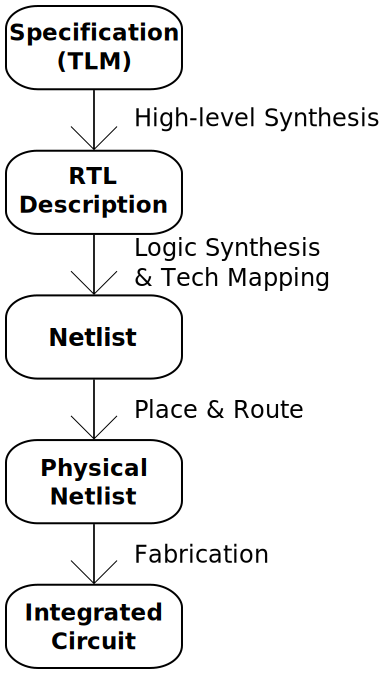
\includegraphics[width=0.5\textwidth]{./figures/designFlow}
}
\caption{Typical hardware design flow.}
\label{fig:cadflow}
\end{figure}
}

%\subsection{The Hardware Verification Imperative}
When moving from one abstraction level of the hardware design process to the 
next, an important issue arises: how can one ensure that the functionality of 
the optimized design matches original spec? 
Bugs in hardware design which are 
not caught early can have costly effects later, such as the need for a 
redesign. Bugs in arithmetic circuits can be especially catastrophic.
One infamous example is the 1994 floating point division (FDIV)
bug that affected the Intel Pentium chip \cite{nicely:FDIV}, 
and subsequently cost the company \$475 million because it was  
discovered after the chip's release. In another more fatal case, during the
Gulf war, an American Patriot Missile battery failed to intercept an incoming
enemy missile due to an arithmetic error \cite{arnold:patriot}.
Since hardware bugs can have significant consequences, 
there has been extensive work in field of hardware verification to find and
eliminate bugs prior to fabrication.

The two main methodologies used in hardware verification are simulation and 
formal verification. \emph{Simulation} checks correctness by applying exhaustive 
assignments to the circuit inputs and verifying correctness of the output. 
This ensures that the circuit performs as designed under all possible 
inputs. Such exhaustive testing is quite effective for smaller circuits. 
However, as the size of the circuit increases, it becomes 
computationally infeasible to simulate all possible test vectors. This is the 
case with Galois field arithmetic circuits, which are commonly very large in 
real-world applications. Often for such large circuits, simulations of a smaller and more 
manageable subset of test vectors are employed to catch bugs. While these tests
can increase confidence in the correctness of the design,  
{\it they do not guarantee correctness} since every data-flow of the design hasn't
been analyzed.
%Such is the case with large Galois field arithmetic circuits, so we instead 
%focus on formal verification. 

\section{Formal Verification}
Instead of simulating input vectors, \emph{formal verification} utilizes 
mathematical theory to reason about the correctness of hardware designs.
%which overcomes some limitations of simulation. 
Formal verification has two main forms: property checking and equivalence 
checking. 

{\it Property checking} (or property verification) verifies
that a design satisfies certain given properties. Property checking is done mainly 
in the form of theorem proving, model checking, or approaches which 
combine the two.
\begin{enumerate}
\item \emph{Theorem proving} \cite{theoremproving:91} requires the existence of
mathematical descriptors of the specification and implementation of the 
circuit. Theorem provers apply mathematical rules to these descriptors to
derive new properties of the specification. In this way, the tool can reduce
a proof goal to simpler sub-goals, which can be automatically verified.
However, generating the initial proof-goal requires extensive guidance from
the user, so there is an overall lack of automation in theorem 
proving.
\item \emph{Model checking} \cite{modelcheck:99} is an approach
to verifying finite-state systems where specification 
properties are modeled as a system of 
logic formulas. The design is then traversed to check if the 
properties hold. If the design is found to violate a
particular property, a counter-example is generated which exercises the
incorrect behavior in the design. Such counter-examples allow the designer
to trace the behavior and find where the error in the design lies.
Modern model checking techniques use the result to automatically refine
the system and perform further checking.
These tools are typically automated, and thus have found widespread 
use in CAD tool suites.
\end{enumerate}

{\it Equivalence Checking} verifies that two different representations of
a circuit design have equivalent functionality. An example of equivalence
checking as it applies to the hardware design flow is shown in
Fig. \ref{fig:equivflow}.

{
\begin{figure}[h]
\centerline{
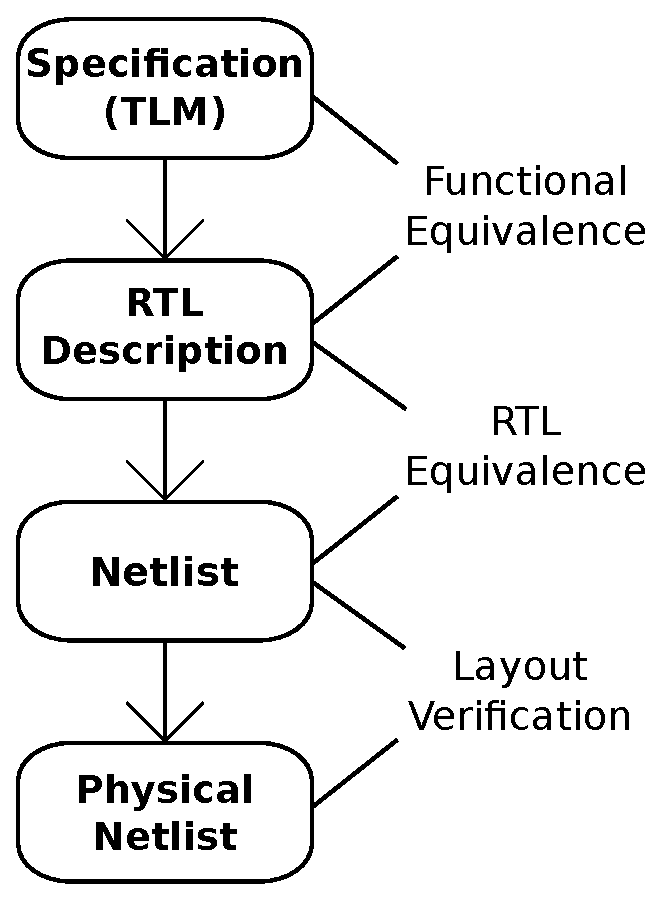
\includegraphics[width=0.5\textwidth]{./figures/designVerification}
}
\caption{Equivalence checking as applied to the hardware design flow.}
\label{fig:equivflow}
\end{figure}
}

There are two major
equivalence checking techniques: graph-based
and satisfiability-based.
\begin{enumerate}
\item \emph{Graph-based} techniques construct a canonical graph 
representation, such as a Binary Decision Diagram (\emph{BDD}) or one of
its many variants, of each circuit. A linear comparison is then conducted to 
determine whether the two graphs are isomorphic. Since the graph 
representation is canonical, the graphs of the two circuits will be 
equivalent if and only if the circuits perform the same function.
\item \emph{Satisfiability} techniques construct a miter of the two circuits,
typically in a graph such as an And-Inverter graph (\emph{AIG}). A
\emph{miter} is a combination of the two circuits with one bit-level output, which 
is only in a "1" state when the outputs of the circuits differ given 
the same given 
input, as shown in Fig. \ref{fig:miter}. 
A satisfiability (\emph{SAT}) tool \cite{csat} 
is then employed to simplify the graph and find a solution to the miter, 
i.e. find an input for which the 
miter output is "1". If a solution is found, this solution acts as a 
counter-example of when the circuit outputs differ; otherwise the circuits
are functionally equivalent.
\end{enumerate}


{
\begin{figure}[h]
\centerline{
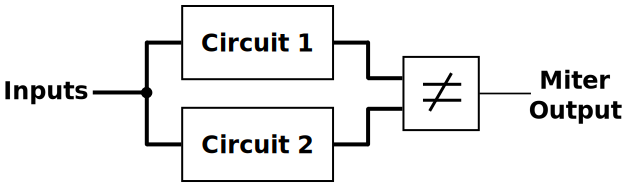
\includegraphics[width=0.8\textwidth]{./figures/betterMiter}
}
\caption{A miter of two circuits.}
\label{fig:miter}
\end{figure}
}

%\subsection{Computer-Algebra Based Formal Verification}
Certain formal verification methods use \emph{computer-algebra} and \emph{algebraic
geometry} techniques based on mathematical theories.
Unlike SAT-based verification, modern algebraic geometry 
techniques do not explicitly solve the constraints to find a solution; 
rather, they reason about the presence or absence of solutions, or explore
the geometry of the solutions.
These methods \cite{Avrunin:CAV} \cite{condrat-tacas07} \cite{gbverify:2007} 
transform the circuit design into a polynomial system. Typically, this system
of polynomials is then used to compute a Gr\"obner basis \cite{gb_book}. 
Computation of Gr\"obner bases allows for 
the easy deduction of important properties of a polynomial system, 
such as the presence or absence of 
solutions. These properties are then leveraged to perform 
verification. Unfortunately, such a computation 
has been shown to be doubly 
exponential in the worst case, and thus these methods have not been 
practical for real-world applications. However, recent
breakthroughs in computer-algebra hardware verification have shown
that it is possible to overcome the complexity of this computation while
still utilizing the beneficial properties of a Gr\"obner bases
\cite{lv:phd}.

\section{Importance of Word-level Abstraction}
Most formal verification techniques can benefit from word-level abstractions 
of the circuits they verify.
Abstraction is defined as state-space reduction, i.e{\text . }abstraction
reduces state-space by mapping the set of states of a system to a smaller 
set of states. Because the new representation contains fewer states, it
is easier to comprehend and thus easier to use. 
Word-level abstraction focuses specifically on abstracting a word-level
representation of a circuit out of a bit-level representation. For example,
a bit-level representation of an integer multiplier is represented by a
collection of Boolean inputs and outputs, whereas a word-level
abstraction hides the underlying logic and represents the circuit as two 
integer inputs and one integer output, e.g. $Z=A\cdot B$. As the bit-size of the
multiplier increases, the logical implementation of the multiplier grows (typically
exponentially) while the word-level abstraction stays the same.

Word-level abstractions have a wide variety applications in formal 
verification. Theorem proving techniques can leverage abstraction as an 
automatic decision procedure or as a canonical reduction 
engine. For example, since RTL is composed of circuit blocks that represent 
the underlying circuit, RTL verification methods can exploit 
abstractions of these blocks.
This is seen in the following RTL verification methods:
\begin{itemize}  
\item Model checking \cite{kroening:model}, 
where an approximation abstraction of RTL blocks is generated and then 
refined.
\item Graph-based equivalence 
checking \cite{WLS} \cite{arditi:bmd}, where abstraction methods are used
to generate a canonical word-level graph representation of the circuit.
\item Satisfiability-based equivalence checking \cite{lpsat}, where 
abstractions are used identify symmetrics and similarities in order to 
minimize the amount of logic that is sent to the 
SAT tool. 
\end{itemize}

Other equivalence checking techniques that employ abstractions 
include satisfiability modulo theory ({\it SMT}) techniques \cite{boolector} \cite{bryant:tacas07}, 
which are similar to SAT except they operate on higher-level data
structures (integers, reals, bit vectors, etc.), as well as 
constraint solving techniques \cite {ms:research} \cite{tew:iccad08}.
In general, RTL equivalence checking approaches would ideally maintain a 
high-level of abstraction while still retaining sufficient lower-level 
functional details  (such as bit-vector size, precision, etc) 
\cite{gupta_survey}.

Word-level hardware abstractions also have applications in RTL and datapath 
synthesis \cite{demicheli:iccad_98} \cite{demicheli:dac_99}
\cite{demicheli:tcad_03}. 
Abstractions of circuits allow for design reuse, which allows for tool-automated 
synthesis of larger circuit blocks.
Since hardware design specifications tend to be word-level, synthesis tools 
can use these larger circuit blocks to generate and optimize the
datapaths and create the RTL of the system. Thus, in order for a circuit to 
be used by these automated synthesis tools, its word-level abstraction must
be known.

Finally, abstractions can also be applied to detect malicious 
modifications to a circuit, potentially inserted as a hardware trojan horse.
Hardware trojans, a relatively new security concern in the hardware 
industry, use certain techniques to add incorrect behavior to a 
design. 
This behavior is only activated under certain rare circumstances that only 
the mal-intent designer has knowledge of.
The behavior is purposely hidden and is very difficult to encounter during 
simulation of the design. A manufactured chip with a subsystem 
that contains a hardware trojan could compromise the entire system in which 
it is used.
In some hardware trojan cases, formal verification techniques may be applied 
to catch a bug in a design and provide a counter-example which exercises it. 
However, it can be difficult to tell whether the bug in the design was 
introduced intentionally of not. On the other hand, word-level abstractions 
of bit-level circuits {\it effectively reverse-engineer the true function 
implemented by the circuit}, which could be used to determine the designer's 
true intention.

\section{Dissertation Objective, Motivation, and Contributions}
This dissertation focuses on abstracting a canonical, 
word-level representation of hardware (bit-level) implementations of 
combinational circuits. The proposed technique is a full abstraction solution which can be 
applied to any arbitrary acyclic combinational circuit. 
It is particularly efficient when applied to Galois field arithmetic circuits.
Using this technique, if the abstraction of the circuit's implementation and its
specification are found, they can be easily compared to determine equivalence.
Implementation of a custom software tool, developed to compute the abstractions, is
also described.

\subsection{Motivating Application}
The motivation for this work comes from applications of Galois field 
arithmetic circuits in elliptical curve cryptography ({\it ECC}) hardware systems.
The main operations of encryption, decryption, and 
authentication in ECC rely on operations performed on elliptic curves, which 
are implemented in hardware as polynomial functions over Galois fields. 
To be applicable in real-world situations, ECC data-paths
should be a minimum of $163$-bits wide, which is the minimum NIST standard, 
up to a recommended size of $571$-bit operand widths. Many non-ECC cryptosystems
have datapaths on the order of $1000$-bits.

A Galois field arithmetic circuit with a datapath size of $k$ 
is built as a Boolean function: $\mathbb{B}^k \rightarrow \mathbb{B}^k$. 
This function is mapped to an operation 
$f:\mathbb{F}_{2^k} \rightarrow \mathbb{F}_{2^k}$ 
over the Galois field $\mathbb{F}_{2^k}$. 
These circuits are custom-built, modular
systems which cannot be synthesized due to their complex nature. Thus, 
formal verification is needed to ensure they operate correctly.

Recent computer-algebra based formal verification techniques have been
able to perform verification of Galois field arithmetic circuits with
a datapath size up to $163$-bits \cite{lv:phd}. Word-level abstractions 
of Galois
field arithmetic circuits could be used to further improve these formal 
verification techniques to allow for verification of larger circuits, as
well as provide the other benefits of word-level abstraction.
However, there is currently no technique for computing word-level 
abstractions of Galois field circuits of any practical size.

{
\begin{figure}[h]
\centerline{
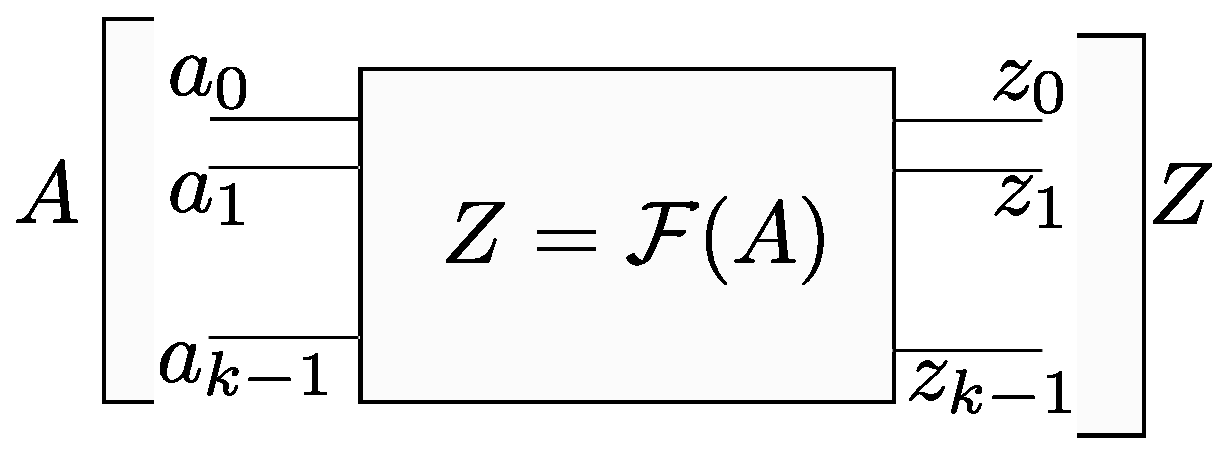
\includegraphics[width=0.5\textwidth]{./figures/interpolate}
}
\caption{Circuit with $k$-bit input $A$ and $k$-bit output $Z$. 
Abstraction to be derived as $Z=\Func(A)$.}
\label{fig:abstractA_Z}
\end{figure}
}

While the motivation comes from the need to verify Galois field arithmetic
circuits, the presented approach can be generalized to be applicable to any
combinational acyclic circuit.
Any such circuit with a $k$-bit input $A$ and a $k$-bit output $Z$, such
as the one shown in Fig. \ref{fig:abstractA_Z}, computes 
$f: \mathbb{B}^k \rightarrow \mathbb{B}^k$ and can thus be analyzed as the
function $f: \Fkk \rightarrow \Fkk$. Over $\Fkk$ this function can be 
represented as the polynomial $Z=\Func(A)$. This is trivially generalized
when there are multiple $k$-bit inputs $A_1,A_2,\dots,A_i$, i.e. $Z=\Func(A_1,\dots,A_i)$.
Now assume the word-size of the input differs from the output, that is the circuit
computes $f: \mathbb{B}^m \rightarrow \mathbb{B}^n$ for $m \neq n$. This can 
be represented as a function over Galois fields as $f: \F_{2^m} \rightarrow \F_{2^n}$.
This function can be analyzed over the field $\Fkk$ such that $\Fkk \supset \F_{2^m}$ 
and $\Fkk \supset \F_{2^m}$, where $k=LCM(m,n)$.

\subsection{Dissertation Contributions}
To solve the problem of word-level abstraction, this dissertation proposes 
a full solution consisting of three main contributions.

\begin{enumerate}
\item A theory for finding the word-level abstraction from a bit-level circuit over Galois fields is created.
The given bit-level circuit implementation is modelled as a system of
polynomials over the field.
This theory is derived using techniques from computer-algebra, notably the theory of
\Grobner basis \cite{pruss:iwls13}.
\item Using this theory, new algorithms based on symbolic computation are developed to 
derive the word-level abstraction. The algorithms are designed to be applicable to 
industry-size arithmetic circuits over Galois fields \cite{pruss:dac14}\cite{sun:date15}.
A complexity analysis of the algorithmic approach is also presented. Furthermore, the
approach is also generalized to make it applicable to arbitrary combinational circuits.
Finally, we show how the approach can be used to exploit the hierarchical structure of
large Galois field multipliers designed over composite fields.
\item A custom software tool implementation of the algorithmic approach is described, including
an analysis of efficient data structures designed for this purpose \cite{pruss:tcad15}.
\end{enumerate}

Experiments show that the proposed solution can abstract canonical, word-level, 
polynomial representations of Galois field arithmetic circuits up to $1024$-bits in
size, while other contemporary approaches are infeasible beyond a $32$-bit designs.


%an 
%approach based on computer-algebra, algebraic geometry - notably the theory of
%{\it Gr\"obner bases} \cite{gb_book} \cite{buchberger_thesis}.
%and {\it elimination ideals} \cite{ideals:book}, as our approach for 
%abstracting canonical word-level representations from bit-level Galois 
%field arithmetic circuits. 
%Computer-algebra techniques easily integrate with 
%Galois field theory and allow for polynomial abstraction of the circuit over 
%the field itself. Thus, if the circuit computes a function over some field $
%\mathbb{F}_{2^k}$, the resulting abstraction is a word-level polynomial 
%function over the same field $\mathbb{F}_{2^k}$. 

%The given bit-level circuit implementation is first modeled as a system of
%polynomials over the field. Using the theory of elimination ideals, we 
%derive an elimination term ordering and prove that by using this ordering we 
%can obtain a canonical word-level representation of a circuit by 
%computing a Gr\"obner basis of the polynomials. However, complexity 
%of the computation of a Gr\"obner basis proves to be prohibitive for circuits
%of practical size. Therefore, we employ a select sub-set of computations 
%from the Gr\"obner basis theory to overcome this complexity and obtain the
%abstraction. We prove that this simpler computation can be 
%performed via a polynomial reduction process, and engineer a custom 
%verification tool for this purpose. Using this approach, we are able to 
%successfully 
%abstract word-level representations of Galois field arithmetic circuits up 
%to $571$-bits, which is the {\it largest recommended NIST standard} for ECC.


\section{Dissertation Organization}
The rest of this dissertation is organized as follows. Chapter
\ref{ch:prev} reviews previous applicable work and highlights their
drawbacks with respect to the canonical, word-level abstraction problem. 
Chapter \ref{ch:prelim} describes the properties of Galois fields, 
$\mathbb{F}_{2^k}$, and explains the process of constructing them.
It also describes how to design arithmetic circuits over such fields, their 
complexities, and the role of these circuits in Elliptic Curve Cryptography.
Chapter \ref{ch:ideals} provides a theoretical background of 
computer-algebra and Gr\"obner bases and explains their application
to Galois fields. 
Chapter \ref{ch:abstract} describes an approach to abstract 
word-level polynomial representations of combinational circuits using a 
Gr\"obner basis computation.
Chapter \ref{ch:improv} improves on this word-level abstraction approach to 
make it applicable to much larger circuits.
Chapter \ref{ch:generalize} generalizes the abstraction approach to make
it applicable to circuits with varying operand word-lengths. It also describes how the 
approach can take advantage of the hierarchy of arithmetic circuits designed over
composite fields.
Chapter \ref{ch:implement} describes the implementation details of a 
custom abstraction tool and gives experimental results of
abstracting large Galois field multiplier circuits.
Chapter \ref{ch:concl} concludes the dissertation and outlines potential future 
research for continuation of this work. 

\chapter{Previous Work}
\label{ch:prev}
\vspace{-0.8cm}
\section{Sequential Equivalence Checking}
As an important component of formal verification for sequential circuits, SEC techniques 
have been developed over decades and widely utilized in both academia and industry. 
The specification of a sequential circuit can be modeled as a (golden model) state machine;
SEC is performed to compare the functionality between the circuit for test and the golden one.
% The n\"aive method to implement SEC is: preload both circuits to the same initial states, 
% and assign their primary inputs to the same values during all clock-cycles.
% This method needs to be operated along with state space traversal,  therefore it is 
% less efficient. Moreover,  most SEC only check the primary outputs/inputs consistency 
% and does not require the 1:1 state correspondence,  so state space traversal is not always necessary.
One way to implement SEC is to create a miter with two circuits to be verified, then 
prove that there exists no sequence of inputs that generates different outputs.

Researchers proposed improvements by using Boolean functions to represent 
a set of states/transitions \cite{coudert2003unified, coudert1990verification},  or by dividing the sequential circuit
into a smaller subcircuit and remodeling the FSM to conditional FSMs \cite{khasidashvili2004theoretical}. IBM created a toolset with 
interfaces that focuses on only the designated initial states and removes redundancies in state space \cite{baumgartner2007scalable}.

Another direction to improve SEC algorithms is to avoid using state space traversal. 
The forward retiming method \cite{van1998sequential} and time-frame merging \cite{stoffel1997record} 
all work on an array of time-frames,  with the assistance of combinational equivalence checking (CEC)
techniques. These techniques require structural similarities between the two circuits.

The most significant difference of sequential circuits from combinational circuits is 
that the outputs of the circuit depend not only 
on the primary inputs, but also on current state. 
The behavioral difference reflects on the structural design of circuits and in 
the existence of memory components such as latches and flip-flops.
In order to test certain properties on some signals across multiple clock-cycles,
the most straightforward method is to propagate those signals throughout 
all clock-cycles. Moreover, for formal verification, all signals on all paths from the circuit
need to be propagated through multiple clock-cycles.
This indicates a time-to-space conversion, where 
 the combinational part of circuit
is copied over several time-frames then connected together.
The procedure is called {\it unrolling} of a sequential circuit, as 
Figure \ref{fig:unrolling} shows.

\begin{figure}[tbp]
\centerline{
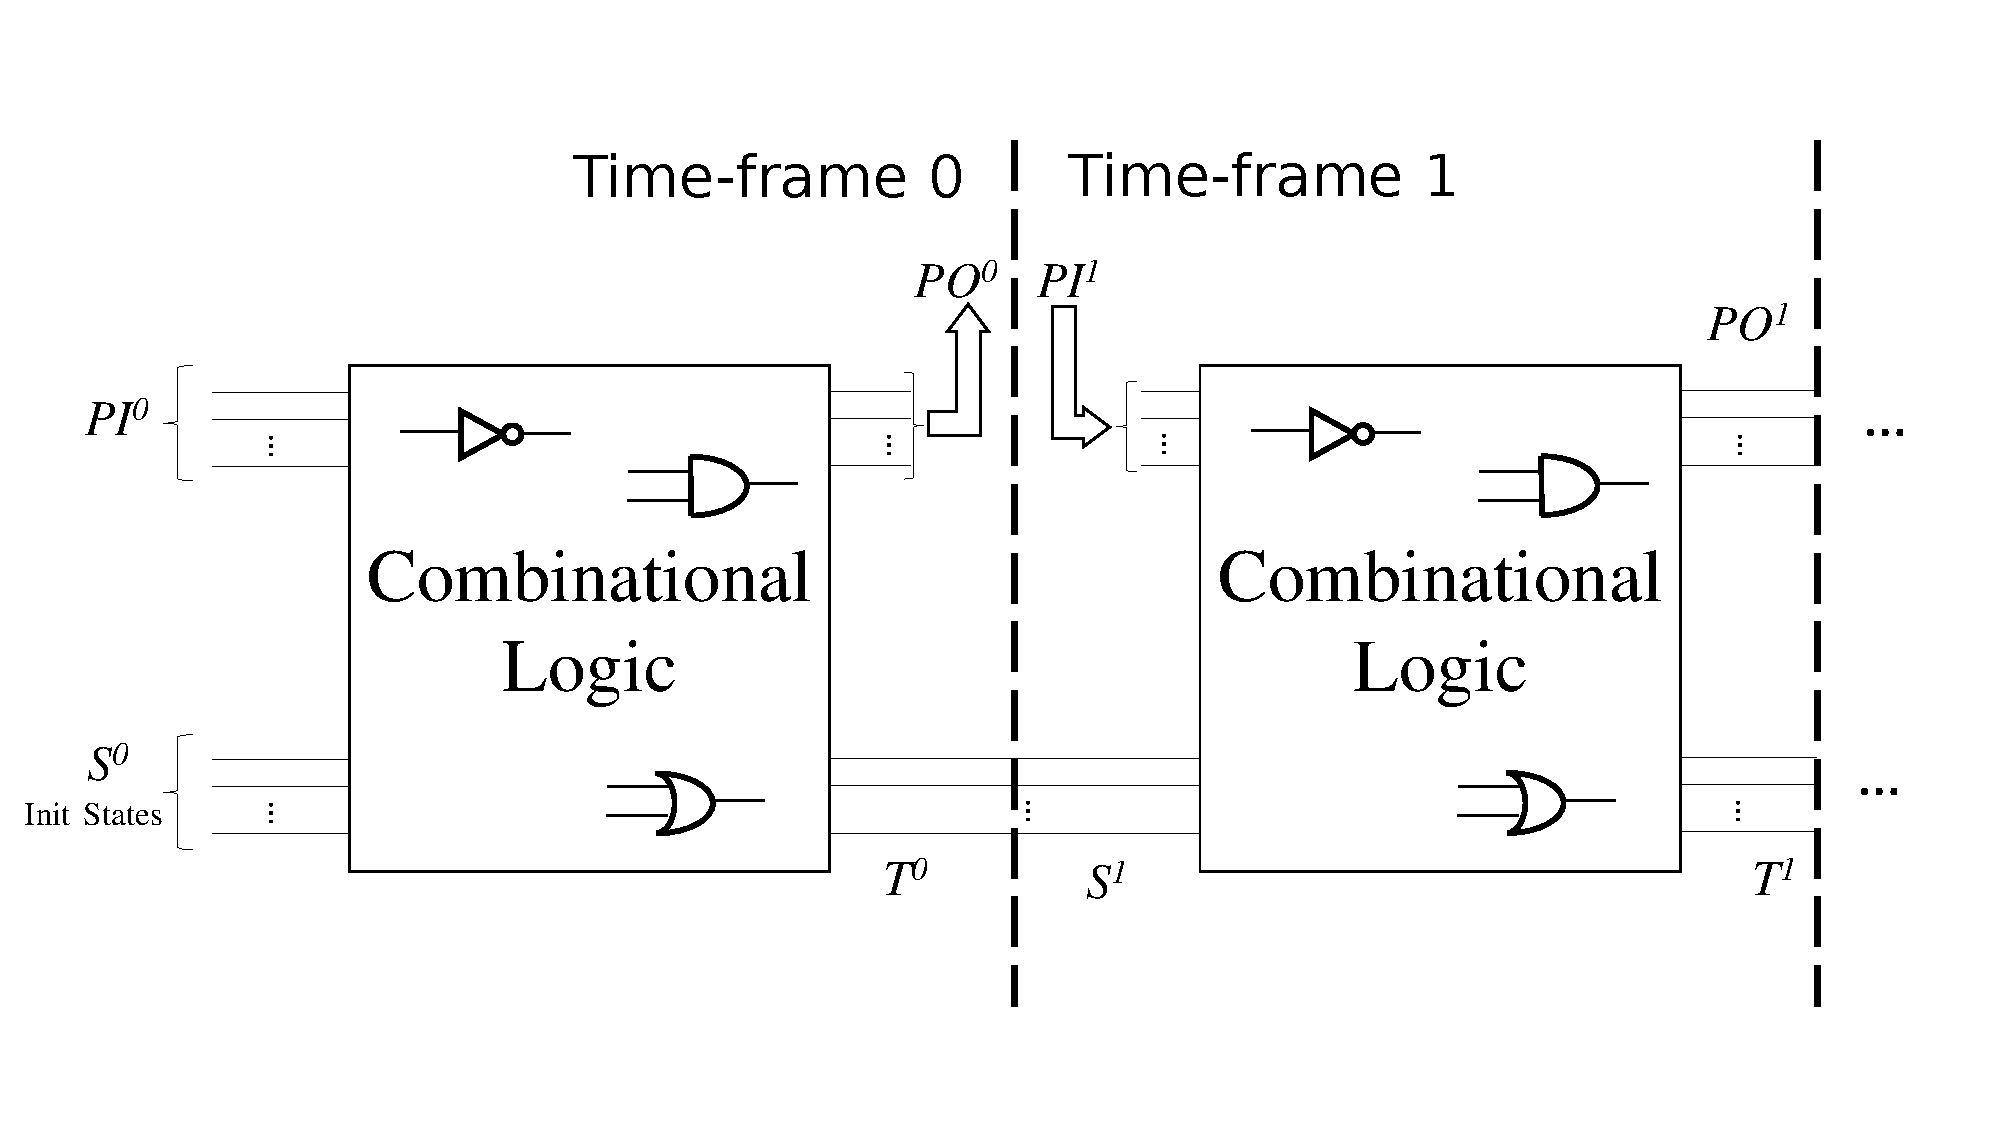
\includegraphics[width=\textwidth]{newfig/unroll.pdf}
}
\caption{The unrolling of a sequential circuit.}
\label{fig:unrolling}
\end{figure}

Unrolling provides a way to transform a sequential circuit into a combinational 
circuit. Therefore,  methods which can be applied to combinational circuit 
verification are also suitable for unrolled sequential circuits. The canonical 
graphical representation of the combinational circuit after unrolling is also 
the canonical representation of the original sequential circuit. For the sequential 
equivalence checking problem, we can also unroll the circuit to be verified and the 
specification to combinational ones, and then perform combinational equivalence checking
techniques \cite{savoj2010combinational}. In the following part we review research and techniques which 
can be applied to unrolled sequential circuits.

\subsection{Canonical Decision Diagrams}
The decision diagrams (DDs) are optimized data structures which can significantly accelerate formal verification.
The most fundamental DD is the Binary DD (BDD), which originates from the 
Shannon's expansion:
\begin{equation}
f(x, y, \dots) = x f_x + x' f_{x'}
\end{equation}
where $f_x = f(x = 1)$ and $f_{x'} = f(x = 0)$ denote the positive and
negative co-factors of $f$ {\it w.r.t.} $x$, respectively.
A BDD is usually represented as a binary tree.
Its ordered and reduced form, the Reduced Ordered Binary Decision Diagram (ROBBD)
\cite{BRYA86}, was the first significant contribution because of its canonicity.  
ROBDDs represent a Boolean function as an
implicit set of points on a canonical directed acyclic graph
(DAG). Manipulation of Boolean functions can then be carried out as
composition operations on their respective DAGs. An example of ROBDD is shown as Figure \ref{fig:BDD}.

Following BDDs,  variants of Shannon's decomposition principle
were explored to develop other functional decision diagrams such as
 FDDs \cite{okfdd}, ADDs \cite{add}, MTBDDs \cite{mtbdd}, and their hybrid 
edge-valued counterparts, HDDs \cite{hdd} and EVBDDs \cite{evbdd}. 
Zero-suppressed BDDs (ZDDs) \cite{minato1993zero,minato1994calculation} use the if-then-else branches
to represent the existence of variables in a cube, and result in lower 
space complexity. They can be used to represent polynomials with integer coefficients.

\begin{figure}[bp]
\centerline{
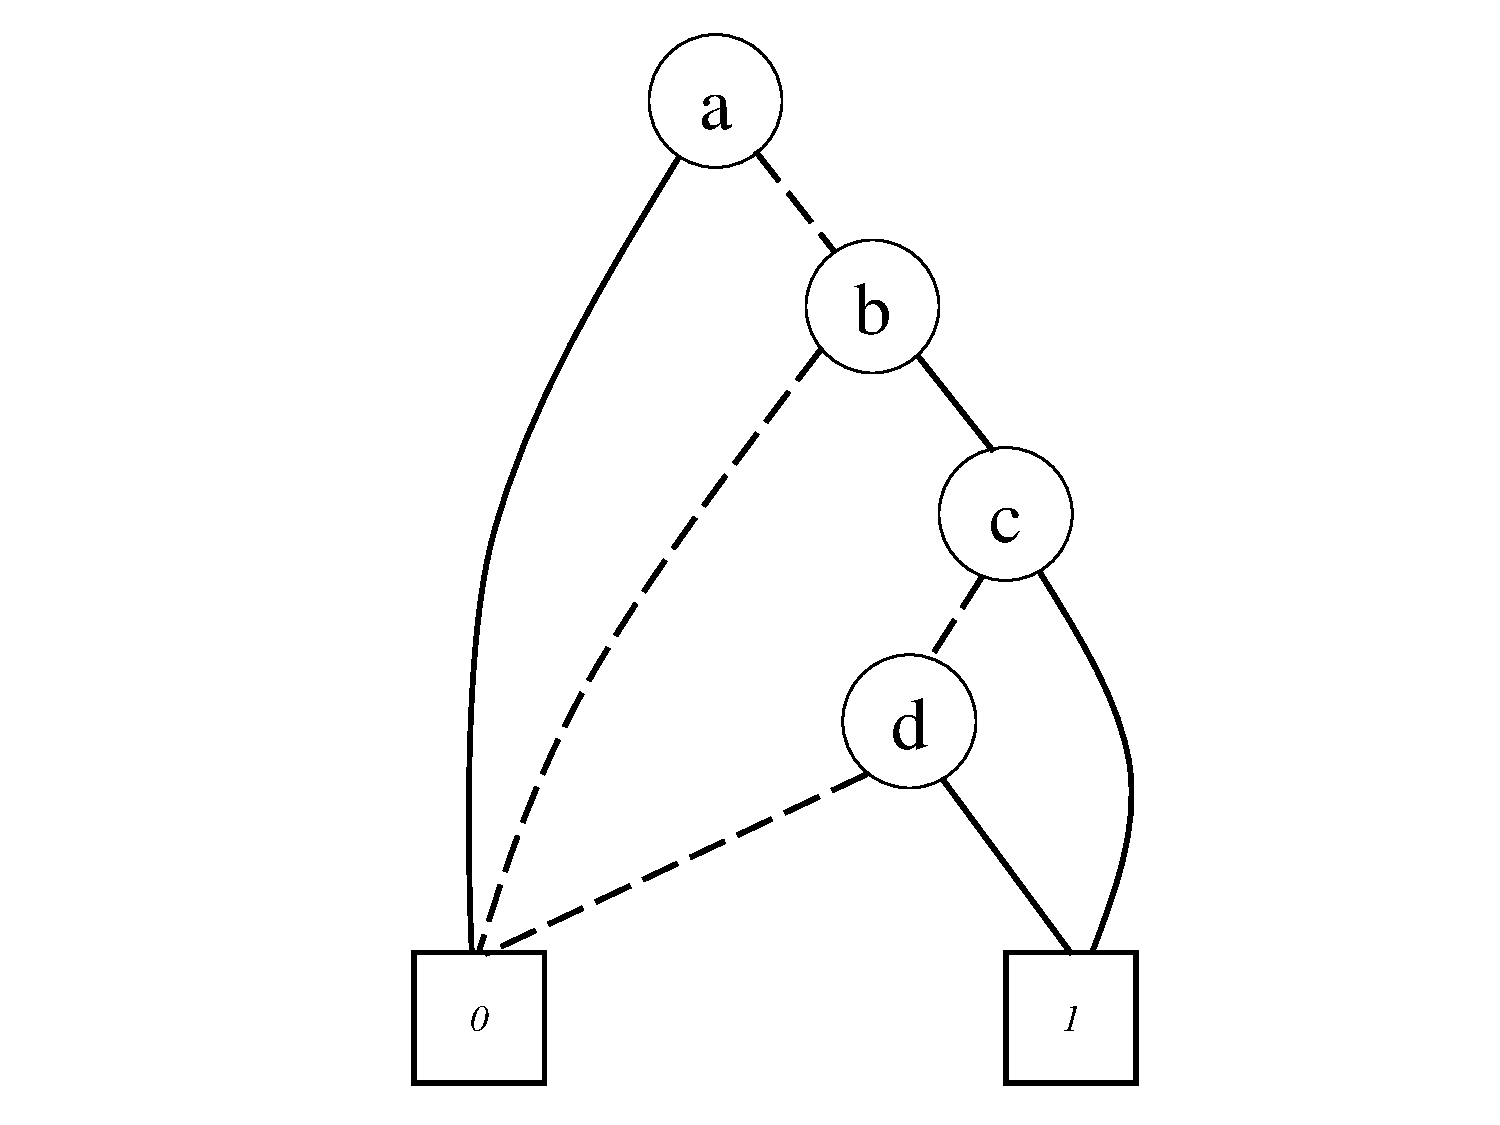
\includegraphics[width=0.45\textwidth]{newfig/BDD.pdf}
}
\caption{ROBDD representing Boolean function $\neg a \land b \land (c\lor d)$ with order $a>b>c>d$.}
\label{fig:BDD}
\end{figure}

The DDs above are all based on bit-level operations. Even in the {\it Word-Level Decision Diagrams}
\cite{WLS}, the decomposition is still point-wise, binary, 
w.r.t. each Boolean variable. These representations do not
serve the purpose of word-level abstraction from bit-level
representations. 

Binary Moment Diagrams (BMDs) \cite{bmd}, and their derivatives K*BMDs
\cite{kbmd} and *PHDDs \cite{phdd}, perform the decomposition of a {\it linear} function
based on its two moments instead of relying on Boolean decomposition. 
MODDs \cite{modd,modd_tcomp} are a DAG representation of the
characteristic function of a circuit over Galois fields $\Fkk$. 
However, MODDs fails to compactly represent large circuits.


Taylor Expansion Diagrams (TEDs) \cite{ted_tcomp} are a
word-level canonical representation of a {\it polynomial expression},
based on the Taylor's series expansion of a polynomial. However, they do
not represent a {\it polynomial function} canonically. 

The use of DDs in traditional formal verification has a lot of advantages. 
For example, DD-based model checking is very efficient as long as the DDs of sequential 
circuit can be setup. The existence of violating states in constructed DDs 
immediately deduces the violation of property. However, when the design gets
larger and larger, the time and space cost of building and storing the diagram 
increases rapidly. In our experiment of verifying a $k$-bit arithmetic circuit 
using ZDDs, when $k$ is larger than 100, the construction of ZDDs occupies 
over $99\%$ runtime of the whole procedure.
\subsection{Combinational Equivalence Checking Techniques}
The CEC problem can be solved using various methods.
Besides using canonical DDs (BDDs
\cite{BRYA86} and their word-level variants \cite{WLS}),
noncanonical representations such as And-Invert-Graph-based (AIG-based) reductions 
\cite{AIG:2002,alanmi:cec:iccad2006} are also very effective. 
Solvers for satisfiability problems (SAT) are good candidates to solve CEC problems,
as long as the miter of two circuits can be described using conjunctive normal form (CNF)
formulas. Applications of SAT on CEC include circuit-SAT solvers \cite{csat}, etc.
If the circuits being compared are structurally highly similar, AIG and circuit-SAT-based
approaches are known to be efficient.
However, when the circuits are functionally equivalent but structurally very dissimilar, none of the 
  contemporary techniques, including quantifier-free bit-vector 
  (QF-BV) theory-based SMT-solvers \cite{Cryptol:fmcad09},
  offer a practical solution.    


Recently integer polynomial based techniques \cite{ciesielski2014function,rolf:date16} have been proposed  to verify the functional 
correctness of integer arithmetic circuits. Their approach formulates the output signature as a polynomial function 
with binary variables and integer coefficients, then rewrites the polynomial by substituting gate output with gate 
inputs. After going through the backward rewriting procedure,  the polynomial
will be composed by only input variables. Then the polynomial is converted to a canonical representation, and compared
with a designated input signature. If they are equivalent, then the arithmetic circuit is successfully verified.
This approach incurs polynomial term explosion during the backward rewriting. The authors proposed a heuristic
to levelize the arithmetic circuit, and substitute several gates' variables at the same time to minimize the risk. However, 
the heuristic proved to be less effective when the inner symmetry of the circuit structure is missing.

% To conclude, automatic formal verification of large {\it
%     custom-designed modulo-arithmetic circuits} largely remains
%   unsolved today.
  
\section{Symbolic Model Checking and Abstraction Refinement}
Model checking is a way to verify certain safety and liveness properties 
in sequential circuits. Symbolic model checking, which avoids using explicit state encoding,
provides more flexibility to reduce the state space and enhance the 
efficiency of model checkers. The implementations of symbolic model checking 
require canonical DDs or SAT solvers \cite{burch1990sequential,burch1991representing,biere1999symbolic}.

Abstraction is a technique to reduce the state space representation by combining states with similar 
characteristics. Sometimes it can effectively lower the number of states that require analysis by orders of magnitude,
without affecting the properties we need to verify. Model checkers then utilize abstracted models 
with interpolation \cite{mcmillan2003interpolation,mcmillan:cav06}.
At first, abstraction was done manually by designers. Clarke {\it et al.} \cite{clarke2000counterexample}
proposed a BDD-based automated abstraction by removing spurious paths from analysis of counterexamples. 
Zhang {\it et al.} \cite{zhang2005design} proposed another abstraction method based on CNF-SAT.
It implemented latch abstraction by removing "irrelevant" latches by analyzing the 
UNSAT core from the $k$-BMC. Jain {\it et al.} \cite{jain2005word} improved the abstraction refinement technique of \cite{clarke2000counterexample},
where they use CNF-SAT to perform the refinement instead of using BDDs. The new approach is applied to verify RTL Verilog
and was known to be successful.

The $k$-BMC with interpolation is a purely incremental model-checking approach, and the interpolation procedure relies
on UNSAT core analysis. To overcome these weaknesses, a hybrid model checker called IC3 is developed 
\cite{bradley2011sat,bradley2011incremental}. IC3 works incrementally to find inductive subclauses
of negations of reached states, meanwhile it is monolithic when computing overapproximations to sets of reachable
states within $1,2,\dots,k$ steps. It is proved to be more efficient than interpolation-based model checking,
although using similar mechanisms.

The above techniques have limitations: they all rely on bit-level information from 
the circuit, which prevents them from being applied to circuits with large datapaths.
Meanwhile, their implementation relies on SAT/BDDs, which is an extension of Boolean 
functions and not compatible with other forms of constraints.

\section{Word-level Techniques Applied to Sequential Circuit Synthesis and Validation}
To better verify word-level designs, word-level verification techniques have been 
explored in recent years. Directly translating bit-vector problems to bit-level 
problems is called {\it bit-blasting}, and usually brings high redundancy and computational complexity in verification.
Attempts to develop pure word-level techniques can be found in
the rich domain of 
theorem proving \cite{arditi:bmd} and bit-vector SMT-solvers
\cite{boolector,cvc3,z3,bitvector98}, automated
decision procedures for Presburger arithmetic \cite{presburger,bultan:mixed_verification}, 
algebraic manipulation techniques 
\cite{devadas:algebraic_manipulation_iccd91}, or the ones based on
term rewriting \cite{AST}, etc.

Polynomial, integer, and other nonlinear representations have also
been researched: Difference Decision Diagrams (DDDs) \cite{ddd-csl99,ddd-mt-98}, interval
diagrams \cite{interval_dd}, interval analysis using polynomials
\cite{polynomial_sanchez99}, {\it etc.} Most of these have found 
application in constraint satisfaction for simulation-based
validation:  \cite{Ritter99,hsat,lpsat,brinkmann:asp-dac,Huang:tcad01,bitvector98}. Among
these, \cite{brinkmann:asp-dac,Huang:tcad01,bitvector98}
have been used to {\it solve} integer modular arithmetic on linear
expressions -- a different application from {\it representing}
finite field modulo-arithmetic on polynomials in a canonical form.   

Uninterpreted function abstraction is also an important category of 
word-level techniques which facilitates word-level model checking.
Usually uninterpreted symbols have no notion of bit-vector-precision. However, these techniques
constrain them 
using functional consistency among the evaluations of word variables
\cite{UF1,UF2,UF3}.


\section{Verification Using Algebraic Geometry}

Symbolic computer algebra techniques have been employed for formal
verification of circuits over $\Z_{2^k}$ and also over
Galois fields $\Fkk$. 
Verification techniques using Gr\"obner bases
\cite{Avrunin:CAV,gbverify:2007,manna:program} are proposed,
but they do not address the problem of high computational complexity to
compute Gr\"obner bases.

Verification of a combinational Galois field arithmetic circuit $C$ against a
polynomial specification $\Func$ has been previously addressed 
\cite{ibm:blueveri,lv:tcad2013,pruss:dac14}. Verification problems in
\cite{ibm:blueveri,lv:tcad2013} are formulated using
Nullstellensatz and decided using the \Grobner basis algorithm.

The paper 
\cite{pruss:dac14} performs verification by deriving a canonical
word-level polynomial representation $\Func$ from the circuit $C$. Their
approach views any arbitrary Boolean function (circuit) $f: \B^k
\rightarrow \B^k$ as a polynomial function $f: \Fkk \rightarrow \Fkk$,
and derives a canonical polynomial representation $\Func$ over
$\Fkk$. They show that this can be achieved by computing a reduced 
\Grobner basis {\it w.r.t.} an {\it abstraction term order} derived from the
circuit. Subsequently, they propose a \underline{r}efinement of this
\underline{a}bstraction \underline{t}erm \underline{o}rder (called
RATO) that enables them to compute the \Grobner basis of a smaller subset
of polynomials. The authors show that their approach can prove the
correctness of up to 571-bit combinational GF multipliers. 

IBM proposed a method to apply algebraic geometry techniques 
to verifying error coding circuits \cite{BLUEVERI}.
Recent papers \cite{rolf:date16,rolf:FMCAD16} provide a way to utilize 
algebraic geometry and GB-based symbolic computing and perform 
equivalence checking on integer arithmetic circuits and floating-point 
arithmetic circuits, respectively.

The use of algebraic geometry
for sequential circuit verification and symbolic model checking has
been presented before. Avrunin presented the
concept of symbolic MC using algebraic geometry in
\cite{Avrunin:CAV}. Later, in \cite{vardi-iasted07}, Vardi presented
GB-algorithms for CTL, LTL, and 
bounded MC over Boolean rings. However, these approaches are a
straightforward transformation of the problem to {\it bit-level}
Boolean GB engines which are used in lieu of BDDs or SAT solvers. All
the concepts of word-level reachability, abstraction-refinement using
interpolation or UNSAT cores, etc., that we desire were not the focus of
\cite{Avrunin:CAV,vardi-iasted07}. 

\section{Concluding Remarks}
From the investigation of previous work, techniques are to be researched that 
can perform the FSM traversal at word level to verify a property excluding spurious 
faults. Meanwhile, many abstraction refinement techniques utilize information from UNSAT cores.
We propose to solve these problems in the context of word-level verification,
with data representation, abstraction, and algorithm execution all carried out 
at word level.

In this dissertation, we propose a purely word-level reachability analysis approach, which has never been done before.
We achieve this by modeling the transition relations, states and the traversal algorithm at word level.
We borrow inspirations from \cite{tim:phd,gao:qe-gf-gb} to perform state space abstraction.
Moreover, we demonstrate applications of our proposed approach to sequential arithmetic verification, which has 
not been done before, either.
Finally, we show algebraic geometry analogs of UNSAT cores of polynomial ideals, and describe algorithms
to extract and refine these cores.

\section{Galois Fields, Polynomial Functions \& Hardware Design}
\label{sec:prelimgf}
%\vspace{-0.035in}

%% We briefly describe the relevant concepts related to Galois fields
%% $\Fkk$; for more details, interested readers may refer to the textbook 
%% \cite{galois_field:mceliece}. 
%% %to put the complexity of the verification problem in perspective, 
%% %to shed some light on the complexity of our design verification, 
%% We also review some VLSI architectures used for Galois field
%% computations \cite{mastro:phd} \cite{acar:1998} \cite{wu:2002}
%% \cite{Knezevic:2008} \cite{eccld} \cite{ecc163}. In our experiments,
%% we have verified custom designs based on these architectures. 

%%%%%%%%%%%%%%%%%%%%%%%%%%%%%%%%%%%%%%%%%%%%%%%%%%%%%%%%%%%%%%%%%%%%%%%%%%%%
%% %\begin{Definition}
%% A finite field, also called a {\bf Galois field}, denoted by $F_q$, is
%% a set of $q$ elements, including two distinguished elements 0 and 1,
%% along with operations $'+'$ and $'\cdot'$ (addition and
%% multiplication) that satisfy the following properties: 
%% \begin{itemize}
%% \item ($F_q, +, 0$) forms an Abelian group.

%% % \begin{itemize}
%% % \item  Closure: $\forall a, b \in F_q, a + b \in F_q$.
%% % \item Associativity: $\forall a, b, c \in F_q, a+(b+c)=(a+b)+c$.
%% % \item Commutativity: $\forall a, b \in F_q, a+b=b+a$.
%% % \item Additive Identity: $\forall a \in F_q, a+0=a$. 
%% % \item Additive Inverse: $\forall a \in F_q$, there is an additive
%% %   inverse element $-a \in F_q$ such that $a+(-a)=0$. 
%% %\end{itemize}

%% \item ($F_q, +, \cdot, 0, 1$) forms a commutative ring with unity.
%% % \begin{itemize}
%% % \item Multiplication closure: $\forall a, b \in F_q, a \cdot b \in
%% %   F_q$.
%% % \item Multiplication Associativity: $\forall a, b, c \in F_q, a \cdot
%% %   (b \cdot c)=(a \cdot b)\cdot c$.  
%% % \item Multiplication Commutativity: $\forall a, b \in F_q, a \cdot b=b \cdot a$. 
%% % \item Multiplication Identity: $\forall a \in F_q, a\cdot 1=a$. 
%% % \item Distributivity: $\forall a, b, c \in F_q, a \cdot (b+c)=(a
%% % \cdot b)+(a \cdot c)$. 
%% % \end{itemize}

%% \item Every non-zero element in $F_q$ has a   multiplicative inverse:
%%   $\forall a \in F_q - \{0\}, \exists a^{-1} \in F_q$ such that $a \cdot
%%   a^{-1}=1$. 

%% \item The number of elements $q$ of the finite field is a
%%   power of a prime integer, i.e. $q = p^k, k \geq 1, p=$ prime. 

%% \end{itemize}
%% %\end{Definition}

A Galois field is a field with a finite number of elements. The number
of elements $q$ of the field is a power of a prime integer --- i.e. $q
= p^k$, where $p$ is a prime integer, and $k \geq 1$ is a positive
integer \cite{galois_field:mceliece}. Galois fields are denoted as
${\mathbb{F}}_{q}$ and also $GF(q =p^k)$. We are interested in fields
where $p = 2$ and $k >1$ --- i.e. {\it   binary Galois extension
  fields} $\mathbb{F}_{2^k}$ --- as they are widely employed in
hardware implementations of cryptography primitives. 

To construct ${\mathbb{F}}_{2^k}$, we take the polynomial ring
${\mathbb{F}}_2[x]$, where ${\mathbb{F}}_{2} = \{0, 1\}$, and an
irreducible  polynomial $P(x) \in {\mathbb{F}}_2[x]$ of degree $k$, and
construct ${\mathbb{F}}_{2^k}$ as ${\mathbb{F}}_2[x] \pmod{   P(x)}$. As a
result, all field operations are performed 
modulo the irreducible polynomial $P(x)$ and the coefficients are
reduced modulo $p=2$. %=2$; due to which $-1 = +1$ over $\Fkk$. 
Any element $A \in {\mathbb{F}}_{2^k}$ can be represented in polynomial
form as $A = a_0 +  a_1 \alpha + \dots + a_{k-1} \alpha^{k-1}$, where
$a_i \in {\mathbb{F}}_2, i = 0, \dots, k-1$, and $\alpha$ is the root of
the irreducible polynomial, {\it i.e.} $P(\alpha)=0$. The field
$\Fkk$ can therefore be construed as a $k$-dimensional vector space
over ${\mathbb{F}}_2$.

%For
%example, $\mathbb{F}_{16} =  \mathbb{F}_2[x] \pmod{ x^4 + x + 1}$. 

%% \debug{
%% The {\it characteristic} of any finite field with
%% unity element $1$ is the least integer $n$ such that $1 + \dots + 1$
%% {\it (n times)} $= 0$. The characteristic of fields of the type
%% ${\mathbb{F}}_{p^k}$ %{\mathbb{F}}_p[x] \pmod{ P(x)}$ 
%% is the prime integer $p$. Since in our
%% case $p = 2$, all fields of the type $\Fkk$, for any given $k$, have 
%% characteristic 2. As a result, all field operations are performed
%% modulo the irreducible polynomial $P(x)$ and the coefficients are
%% reduced modulo $p=2$; due to which $-1 = +1$ over $\Fkk$. 
%% }

%% Any element $A \in \mathbb{F}_{2^k}$ can be represented in polynomial
%% form as $A = a_0 +  a_1 \alpha + \dots + a_{k-1} \alpha^{k-1}$, where
%% $a_i \in \mathbb{F}_2, i = 0, \dots, k-1$, and $\alpha$ is the root of
%% the irreducible polynomial, {\it i.e.} $P(\alpha)=0$. The field
%% $\Fkk$ can therefore be construed as a $k$-dimensional vector space
%% over $\mathbb{F}_2$.



\begin{Example}\label{ex:1}
Let us construct ${\mathbb{F}}_{2^4}$ as ${\mathbb{F}}_2[x] \pmod{
  P(x)}$, where $P(x)=x^4+x^3+1 \in {\mathbb{F}}_2[x]$ is an
irreducible polynomial of degree $k =4$. Let $\alpha$ be the root of
$P(x)$, i.e. $P(\alpha)=0$.  Any element $A \in {\mathbb{F}}_2[x]
\pmod{ x^4 + x^3 + 1}$ has a representation of the type: $A = a_3 x^3
+ a_2 x^2 +  a_1 x + a_0$ where the coefficients $a_3, \dots, a_0$ are
in ${\mathbb{F}}_2 = \{0, 1\}$. Since there are only 16 such
polynomials, we obtain 16 elements in the field
${\mathbb{F}}_{16}$. Each element in can then be viewed as a 4-bit
vector over ${\mathbb{F}}_2$: ${\mathbb{F}}_{16}=\{(0000),(0001),
\dots (1110),(1111)\}$.  Each element also has an exponential
representation; all three representations are shown in Table
\ref{tab:gfelement}. For example, consider the element $\alpha^{12}$.
Computing $\alpha^{12} \pmod{ \alpha^4+\alpha^3+1} = \alpha + 1
= (0011)$; hence we have the three equivalent representations. 

\vspace{-0.1in}
\begin{table}[h]
\begin{center}
{\small
\caption{Bit-vector, Exponential and Polynomial representation of
elements in  ${\mathbb{F}}_{2^4} = {\mathbb{F}}_2[x]
\pmod{x^4+x^3+1}$}\label{tab:gfelement}  
\begin{tabular}{|c|c|c||c|c|c|} 
\hline
$a_3a_2a_1a_0$ & Exponential & Polynomial     &$a_3a_2a_1a_0$ & Exponential & Polynomial  \\
\hline
$0000$        & $0$         & $0$            & $1000$ & $\alpha^3$ &  $\alpha^3$\\
\hline
$0001$        & $1$         & $1$            & $1001$ & $\alpha^4$ & $\alpha^3 + 1$\\
\hline
$0010$        & $\alpha$    & $\alpha$       & $1010$ & $\alpha^{10}$&$\alpha^3 + \alpha$  \\
\hline
$0011$        & $\alpha^{12}$& $\alpha + 1$   & $1011$ & $\alpha^5$ & $\alpha^3+\alpha+1$\\
\hline
$0100$        & $\alpha^2$  & $\alpha^2$     &  $1100$ & $\alpha^{14}$ & $\alpha^3 + \alpha^2$\\
\hline
$0101$        & $\alpha^9$   &$\alpha^2 + 1$ & $1101$  &$\alpha^{11}$  & $\alpha^3+\alpha^2+1$\\
\hline
$0110$        & $\alpha^{13}$& $\alpha^2 + \alpha$ & $1110$ & $\alpha^8$& $\alpha^3+\alpha^2+\alpha$\\
\hline
$0111$        &$\alpha^7 $ & $\alpha^2+\alpha+1$ & $1111$ &$\alpha^6$ & $\alpha^3+\alpha^2+\alpha+1$\\
\hline
\end{tabular}
}
\end{center}
\end{table}
\end{Example}




%%%%%%%%%
{\bf Polynomial Functions $f: \Fkk \rightarrow \Fkk$:} 
Arbitrary mappings among $k$-bit vectors can be constructed; each such
mapping generates a function $f: \B^k \rightarrow \B^k$. Since every
$k$-bit vector can be construed as an element in $\Fkk$ (as shown in
the above example), every such function corresponds to a function over
Galois fields: $f: \Fkk \rightarrow \Fkk$. Every such function is also
a polynomial function. 

\begin{Theorem}
From \cite{ff:1997}: 
Let $\Fq$ be a Galois field of $q$ elements where $q$ is a power of a
prime integer. Any  function $f: \Fq \to \Fq$ is a polynomial function
over $\Fq$, that is there exists a polynomial $\F \in \Fq [x]$ such
  that $f(a) = \F(a)$, for all $a \in \Fq$. 
\end{Theorem}

By analyzing $f$ over each of the $q$ points, one can apply
{\bf Langrange's interpolation formula} and interpolate a polynomial
$\F(x) = \sum_{k=1} ^q  \frac{ \prod_{i \neq k}  (x -x_i)}{\prod_{i \neq k}
  (x_k -x_i)} \cdot f(x_k)$, which is a polynomial of degree at 
most $q-1$ in $x$. One can easily see that $\F(a)=f(a)$ for all $a \in
\Fq$, and $\F(x)$ is therefore the polynomial function representation
of $f$. 

\begin{Example} {\it
Let $A = \{a_2, a_1, a_0\}$ and $Y = \{y_2, y_1,
y_0\}$ be 3-bit vectors.  Consider the function $Y[2:0] = A[2:0]
>> 1$, i.e. a {\bf bit-vector right shift} operation on $A$. 
The function maps as follows:

\begin{center}
{\small
\begin{tabular}{c|ccc|c||c|ccc|c}
$\{a_2a_1a_0\}$  & $A$ &$\rightarrow$& $\{y_2y_1y_0\}$ &$Y$ &
  $\{a_2a_1a_0\}$  &$A$&$\rightarrow$& $\{y_2y_1y_0\}$ &$Y$\\
\hline
000  &0 &$\rightarrow$& 000 & 0 & 100  &$\alpha^2$ &$\rightarrow$& 010 &  $\alpha$ \\
001  &1 &$\rightarrow$& 000 & 0 & 101  &$\alpha^2 + 1$ &$\rightarrow$&010 & $\alpha$ \\
010  &$\alpha$ & $\rightarrow$ & 001& 1 & 110  &$\alpha^2 + \alpha$&$\rightarrow$& 011 &$\alpha + 1$ \\   
011  &$\alpha + 1$ &$\rightarrow$& 001 &1 & 111& $\alpha^2 + \alpha + 1$ &$\rightarrow$& 011 &$\alpha + 1$\\
\hline
\end {tabular}
}
\end{center}

If we model this function as $f: {\mathbb{Z}}_{8} \rightarrow
{\mathbb{Z}}_{8}$, then using the results of \cite{singmaster}
\cite{chen_95} \cite{chen_96}, we deduce that this function is not a
polynomial function over ${\mathbb{Z}}_{8}$. However, applying
Largange's interpolation formula over ${\mathbb{F}}_{2^3}$, we obtain
the following polynomial function representation, $Y =
(\alpha^2+1)A^4+(\alpha^2+1)A^2$, where $P(\alpha) = \alpha^3 +
\alpha + 1 = 0$. 
}
\end{Example}

An important property of Galois fields is that for all elements $A \in
{\mathbb{F}}_q, A^q = A$, and hence $A^q - A =  0.$ Therefore, the
polynomial $x^q -x$ {\it vanishes} on all points in
$\Fq$. Consequently, any polynomial $\F(X)$ can be reduced $\pmod{ X^q
  - X}$ to obtain a canonical representation $\F(X) \pmod{X^q - X}$
with degree at most $q-1$. Such {\it vanishing polynomials} will form
an important part of our ideal membership formulation.  


\begin{Definition}
Any function $f: \Fq^d \to \Fq$ has a unique canonical representation
(UCR) as polynomial $\F \in \Fq[x_1,\dots, x_d]$ such that all its 
nonzero monomials are of the form $x_1^{i_1}\cdots x_d^{i_d}$ where $0
\leq i_j \leq q-1$, for all $j=1, \ldots d$.
\end{Definition}


\subsection{Hardware Implementations of Galois Field Arithmetic}
% Operations Over $\mathbb{F}_{2^k}$}

{\bf Point Addition over Elliptic Curves:} The main operations of
encryption, decryption and authentication in elliptic curve
cryptography (ECC) rely on {\it point additions} and {\it doubling}
operations on elliptic curves designed over Galois fields. 
%Point multiplication involves a series of addition and doubling of
%points on the elliptic curve. % -- this, in turn, requires finite
%field multiplications.  
%A drawback of traditional approaches is that they require
%point multiplication is that each point addition and doubling 
In general, this requires computation of multiplicative inverses over
the field - which is expensive. Modern approaches represent
the points in projective coordinate systems, {\it e.g.}, the
L$\acute{o}$pez-Dahab (LD) projective coordinate \cite{eccld},
%\cite{ecc:software},
which eliminates the need for multiplicative inverses and improves the
efficiency of these operations. 

%%%

%% \begin{Example}
%% {\it 
%% Consider point addition in L$\acute{o}$pez-Dahab (LD) projective
%% coordinate. Given an elliptic curve: $Y^2 + XYZ = X^3Z + aX^2Z^2 +
%% bZ^4$ over $\mathbb{F}_{2^k}$,   where $X,Y,Z$ are $k$-bit vectors
%% that are elements in $\mathbb{F}_{2^k}$ and similarly, $a, b$ are
%% constants from the field.   Let ($X_3$, $Y_3$, $Z_3$) = ($X_1$, $Y_1$,
%% $Z_1$) + ($X_2$, $Y_2$, $1$)  represent point addition over the
%% elliptic curve.  Then $X_3$, $Y_3$, $Z_3$ can be computed as follows: 

%% \begin{align*}
%% A &= Y_2 \cdot Z_1^2 + Y_1 \\
%% B &= X_2 \cdot Z_1 + X_1 \\
%% C &= Z_1 \cdot B \\
%% D &= B^2 \cdot(C + a Z_1^2) \\
%% Z_3 &= C^2 \\
%% E &= A \cdot C  \\
%% X_3 &= A^2 + D + E  \\
%% F &= X_3 + X_2 \cdot Z_3 \\
%% G &= X_3 + Y_2\cdot Z_3 \\
%% Y_3 &= E\cdot F + Z_3 \cdot G \\
%% \end{align*}
%% }
%% \end{Example}

\begin{Example}
{\it 
Consider point doubling in LD projective coordinate system. Given an
elliptic curve: $Y^2 + XYZ = X^3Z + aX^2Z^2 + bZ^4$.  
Let  ($X_3$, $Y_3$, $Z_3$) = 2($X_1$, $Y_1$, $Z_1$), then $X_3, Y_3,
Z_3$ can be computed as: $X_3 = X_1^4 + b \cdot Z_1^4; ~~Z_3 = X_1^2
\cdot Z_1^2; ~~Y_3 = b Z_1^4 \cdot Z_3 + X_3 \cdot (aZ_3 + Y_1^2 +
bZ_1^4 )$. 
}
\end{Example}

The multiplication and iterative squaring operations in the above
computation are usually implemented using custom-designed Galois field
multipliers, such as the Mastrovito \cite{mastro:1989}, Montgomery
\cite{acar:1998}, Barrett multipliers \cite{Knezevic:2008}, or
composite-field multipliers \cite{cfmulti:1996} --- which are, in
turn, hierarchically designed.  For example, Montgomery reduction (MR)
computes: $MR(A,B)=A\cdot B \cdot R^{-1} \pmod {P(x)}$, 
where $A,B$ are $k$-bit inputs, $R$ is suitably chosen as
$R={\alpha}^k$, $R^{-1}$ is multiplicative inverse of $R$ in
${\mathbb{F}}_{2^k}$, and $P(x)$ is the irreducible polynomial.
Since Montgomery reduction cannot directly compute $A\cdot B \pmod
{P(x)}$, we need to pre-compute $A\cdot R$ and $B\cdot R$, as shown in
Figure \ref{fig:mm4}.   

\begin{figure}[hbt]
	\begin{center}
	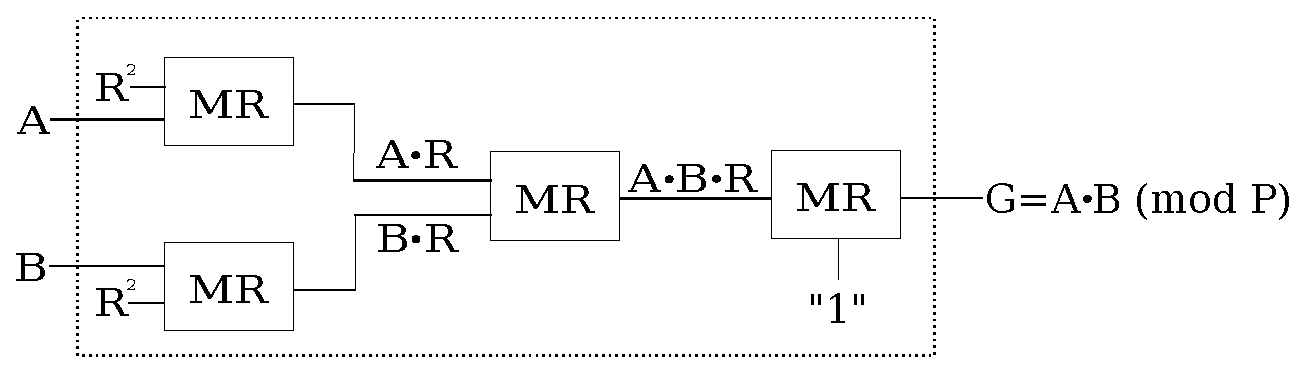
\includegraphics[scale=0.4]{new_mmcircuit.eps}
	\end{center}
	\caption{{\it Montgomery} multiplication over $\mathbb{F}_{2^k}$
          using four Montgomery reductions.}
	\label{fig:mm4}
\end{figure}

Given a hierarchically designed Montgomery multiplier, we will first
extract polynomials $AR, BR, ABR$ from the sub-circuit blocks. By
analyzing the interconnection of these sub-circuits at word-level, we
can then apply our approach at a higher-level, to extract the function
of the entire circuit. Performing such operations hierarchically, we
will apply our approach to reverse-engineer point-addition circuits
designed using a variety of such Galois field adder and multiplier
circuits.  

\section{Computer Algebra Preliminaries}
\label{sec:ideals}

%We review basic commutative algebra concepts related
%to ideals, varieties, Nullstellensatz and Gr\"obner bases, and their 
%application over Galois fields; the material is referred from
%\cite{ideals:book} \cite{gb_book} and \cite{gao:gf-gb-ms}. 

We denote a Galois field of $q$ elements by $\Fq$, where $q = 2^k$ in
our case. Let $\Fq[x_1,\dots, x_d]$ be
the polynomial ring over $\Fq$ with indeterminates $x_1, \dots, 
x_d$. A {\it monomial} in variables $x_1, \cdots, x_d$ is a product of
the form $X = x_1^{\alpha_{1}}\cdot x_2^{\alpha_{2}}\cdots
x_d^{\alpha_{d}}$, where $\alpha_i \geq 0, i\in \{1, \dots, d\}$. A
{\it polynomial} $f \in \Fq[x_1,\dots, x_d], f\neq 0$, is 
written as a finite sum of terms $f = c_1 X_1 + c_2 X_2 + \dots + c_t
X_t$.  Here $c_1, \dots, c_t$ are coefficients and $X_1, \dots, X_t$
are monomials. To systematically manipulate the polynomials, a {\it
  monomial  ordering} $>$ is imposed such that $X_1 > X_2 > \dots >
X_t$. 
%It is a  well-ordering on the set of all monomials such that
%multiplication with a monomial preserves the
%ordering\footnote{Lexicographic ({\it     lex}), degree-lexicographic
%  ({\it deglex}), degree-reverse-lexicographic ({\it degrevlex}) are
%  examples of monomial orderings.}. 
Subject to such an ordering, $lt(f) = c_1 X_1,  ~lm(f) = X_1, ~lc(f) =
c_1$, are the {\it leading   term}, {\it  leading monomial} and {\it
  leading coefficient} of $f$, respectively. Similarly, tail($f$) =
$c_2X_2 + \dots + c_t X_t$. Division of a polynomial $f$ by polynomial
$g$ gives remainder polynomial $r$, denoted $f \xrightarrow{g}_+ r$.
Similarly, $f$ can be reduced (divided) w.r.t. a set of polynomials
$F = \{f_1, \dots, f_s\}$ to obtain a remainder $r$, denoted $f
\stackrel{F} {\textstyle \longrightarrow}_+ r$, such that no term in
$r$ is divisible by the leading term of any polynomial in $F$.  

%{\bf Polynomial reduction:} Let $f, g$ be polynomials. If a non-zero
%term $cX$ of $f$ is divisible by the leading term of $g$, then we say
%that $f$ {\it reduces} to $r$ modulo $g$, denoted $f
%\stackrel{g}{\textstyle\longrightarrow} r$, where $r = f - {cX   \over
%  lt(g)} \cdot g$. 

{\bf Ideals and varieties:} An {\it ideal} $J$ generated by
polynomials $f_1, \dots, f_s \in \Fq[x_1,\dots, x_d]$ is:
$J = \langle f_1, \dots, f_s \rangle = \{\sum_{i=1}^{s}
h_i\cdot f_i: ~h_i \in \mathbb{F}[x_1,\dots,  x_d]\}.$  The
polynomials $f_1, \dots, f_s$ form the basis or generators of
$J$. 

Let $\mathbf{a} = (a_1, \dots, a_d) \in \Fq^d$ be a point, and
$f \in \Fq[x_1,\dots, x_d]$ be a polynomial. We say that $f$
{\it vanishes} on $\mathbf{a}$ if $f(\mathbf{a}) = 0$. 
For any ideal $J = \langle f_1, \dots, f_s \rangle \subseteq
\Fq[x_1,\dots, x_d]$, the {\it affine variety} of $J$ over
$\Fq$ is:
$V(J) = \{\mathbf{a} \in \mathbb{F}^d: \forall f \in
J, f(\mathbf{a}) = 0\}.$ In other words, the variety corresponds to
the set of all solutions to $f_1 = \dots f_s = 0$. 
%If $J = \langle
%f_1, \dots, f_s \rangle = \langle g_1, \dots, g_t \rangle$, then $V(J)
%= V(f_1, \dots, f_s) = V(g_1, \dots, g_t)$. 

%%%% Florian says: I_{\mathbb{F}}(V)....


%\begin{Definition}
For any subset $V$ of $\Fq^d$, the ideal of polynomials that
vanish on $V$, called the {\it vanishing ideal of $V$}, is defined as: 
$I(V) = \{f\in \Fq[x_1,\dots, x_d]: \forall
\mathbf{a} \in V, f(\mathbf{a}) = 0\}.$
%\end{Definition}
%\begin{Proposition}
%\label{prop:finIV}
If a polynomial $f$ vanishes on a variety $V$, then $f \in I(V)$. 
%\end{Proposition}


%% \vspace{-0.1in}
%% \subsection{Radicals and Nullstellensatz}
%% \begin{Definition}
%% \label{radical}
%% Let $J \subset \mathbb{F}[x_1,\dots, x_d]$ be an ideal. The {\it
%%   radical of $J$} is defined as $\sqrt{J} = \{f \in
%% \mathbb{F}[x_1,\dots, x_d]: \exists m \in \mathbb{N}, f^m \in
%% J\}$. 
%% \end{Definition}

%% When $J = \sqrt J$, then $J$ is said to be a {\it radical
%%   ideal}. Moreover, $I(V)$ is a radical ideal. The Strong 
%% Nullstellensatz establishes the correspondence between radical ideals 
%% and varieties.  

%% \begin{Theorem}
%% {\it Strong Nullstellensatz} \cite{gb_book}:  
%% Let $\mathbb{F}$ be an algebraically closed field, and let $J$
%% be an ideal in $\mathbb{F}[x_1,\dots, x_d]$. Then we have $I(V(J)) =
%% \sqrt{J}$. 
%% \end{Theorem}

%% We are concerned with Galois fields, which are not algebraically
%% closed. When a field $\mathbb{F}$ is not algebraically closed, then
%% the above result can be suitably applied over the algebraic closure of
%% $\mathbb{F}$.    

%% %%%% reinforce I_{\mathbb{F}}(---) 

%% \begin{Corollary}
%% \label{cor:nullsatz}
%% Let $\mathbb{F}$ be an arbitrary field and $J$ be an ideal in
%% $\mathbb{F}[x_1,\dots, x_d]$. Let $\overline{\mathbb{F}}$ denote the
%% algebraic closure of $\mathbb{F}$, and let
%% $V_{\overline{\mathbb{F}}}(J)$ denote the variety of $J$ over
%% $\overline{\mathbb{F}}$. Then $I_{\mathbb{F}}(V_{\overline{\mathbb{F}}}(J)) =
%% \sqrt{J}$.     
%% \end{Corollary}


\subsection{Strong Nullstellensatz over Galois Fields}

Our problem formulation is derived from Nullstellensatz, which admits
a special form over Galois fields. We state the following results of
Nullstellensatz over Galois fields, proofs of which can be found in
\cite{gao:gf-gb-ms}.   

%\begin{Proposition}
Let ${\mathbb{F}}_q$ be a Galois field of $q$ elements. For all elements
$A \in \Fq$, we have $A^q - A = 0$. Therefore, for a polynomial $x^q -
x$, we have $V(x^q - x) = \Fq$.
%\end{Proposition}
The polynomials of the form $\{x^q - x\}$ are called the {\it
  vanishing polynomials} of the field. Let $F_0 = \{x_1^q - x_1,
\dots, ~x_d^q - x_d\}$, then $J_0 = \langle x_1^q - x_1, \dots, x_d^q
- x_d\rangle$ is the ideal of all vanishing polynomials in
$\mathbb{F}_q[x_1,\dots,   x_d]$. Below, we use the concept of sum of
ideals: given ideals $I_1 = \langle f_1, \dots, f_s \rangle$ and $I_2
= \langle g_1, \dots, g_t \rangle$, then ideal $I_1 + I_2 = \langle
f_1, \dots, f_s, g_1, \dots, g_t\rangle$. 

%% \begin{Lemma}
%% \label{lemma:radical}
%% From \cite{gao:gf-gb-ms}: For any ideal $J \subseteq
%% \mathbb{F}_q[x_1,\dots, x_d]$, $J + J_0 = J + \langle x_1^q - x_1,
%% \dots, ~x_d^q - x_d\rangle$ is radical. In other words, $\sqrt{J +
%%   J_0} = J + J_0$. 
%% \end{Lemma}

%% The above is a very powerful result, as it implies that any ideal $J
%% \in \Fq[x_1, \dots, x_d]$ can be easily turned into a radical ideal by
%% adding $J_0$, without changing the zero-set $V(J)$ over $\Fq$. And,
%% based on the above, the following result can be easily deduced:

\begin{Theorem} %\cite{gao:gf-gb-ms}
\label{thm:strong-nullsatz-fq}
{\it Strong Nullstellensatz over $\Fq$:} For any Galois field $\Fq$,
let $J \subseteq \Fq[x_1,\dots,   x_d]$ be an ideal, and let 
$J_0 = \langle x_1^q - x_1, \dots, x_d^q - x_d\rangle$ be
the ideal of all vanishing polynomials. Let $V_{\Fq}(J)$ denote the
variety of $J$ over $\Fq$.  Then, $I(V_{\Fq}(J)) = J + J_0 = J +
\langle  x_1^q - x_1, \dots, ~x_d^q - x_d\rangle$.  
\end{Theorem}


%% \begin{proof}
%% Let $\overline{{\mathbb{F}}_q}$ denote the algebraic closure of
%% $\Fq$. Therefore, $\overline {\mathbb{F}_{q}} \supset
%% \mathbb{F}_{q}$, and we have:

%% \begin{eqnarray}
%% V_{\mathbb{F}_{q}}(J) &= & V_{\overline {\mathbb{F}_{q}}}(J) \cap \mathbb{F}_{q}^d  \nonumber \\
%%                    &= & V_{\overline {\mathbb{F}_{q}}}(J) \cap  V_{\mathbb{F}_{q}}(J_0)  \nonumber \\
%%                    &= & V_{\overline {\mathbb{F}_{q}}}(J) \cap
%% V_{\overline{\mathbb{F}_{q}}}(J_0) \nonumber  \\ 
%%                    &= & V_{\overline {\mathbb{F}_{q}}}(J+J_0) \nonumber
%% \end{eqnarray}

%% Therefore, $I(V_{\Fq}(J)) = I(V_{\overline
%%   {\mathbb{F}_{q}}}(J+J_0)) = \sqrt{J + J_0}$, from Corollary
%% \ref{cor:nullsatz}. Moreover, Lemma \ref{lemma:radical} says that $(J
%% + J_0)$ is radical, so $\sqrt{J + J_0} = J + J_0$. Consequently, we
%% have that $I(V_{\Fq}(J)) = J + J_0$. 
%% \end{proof}

\subsection{Gr\"obner Basis of Ideals} 

An ideal $J$ may have many different generators: it is
possible to have sets of polynomials $F = \{f_1, \dots, f_s\}$ and $G
= \{g_1, \dots, g_t\}$ such that $J = \langle f_1, \dots, f_s \rangle
= \langle g_1, \dots, g_t\rangle$ and $V(J) = V(f_1, \dots, f_s) =
V(g_1, \dots, g_t)$.  Some generating sets are ``better''
than others, i.e. they are a better representation of the ideal. A
{\it Gr\"obner basis} is one such representation which allows to solve
many polynomial decision questions. 

\begin{Definition} \label{def:gb}
$\bf{\left[Gr\ddot{o}bner\ Basis\right]}$ [From \cite{gb_book}] For
a monomial ordering $>$, a set  of non-zero polynomials $G =
\{g_1,g_2,\cdots,g_t\}$ contained in an ideal $J$, is called a
Gr\"{o}bner basis for $J$ $\iff$ 
$\forall f \in J$, $f\neq 0$, there exists $i \in \{1,\cdots, t\}$ such
that $lm(g_i)$ divides $lm(f)$; i.e., $G = GB(J)
\Leftrightarrow\  \forall f \in J : f \neq 0, \exists g_i \in G :
lm(g_i)\mid lm(f)$. 
\end{Definition}

Gr\"obner bases theory 
provides a {\it decision procedure to test for membership in an
ideal}. As a consequence of Definition \ref{def:gb}, the set $G$ is a
Gr\"obner basis of ideal $J$, if and only if for all $f \in J$,
dividing $f$ by polynomials of $G$ gives  0 remainder:  $G = GB(J)
\iff \forall f\in J, f \stackrel{G}{\textstyle\longrightarrow}_+ 0$. 

Buchberger's algorithm \cite{buchberger_thesis},
shown in Algorithm \ref{alg:gb},  computes a Gr\"obner
basis over a field. Given polynomials $F = \{f_1, \dots, f_s\}$, 
the algorithm computes the Gr\"obner basis $G = \{g_1, \dots, 
g_t\}$.
% such that ideal $I = \langle f_1, \dots, f_s\rangle = \langle g_1,
% \dots, g_t\rangle$. 
In the algorithm,  

\begin{equation}
       Spoly(f,g)=\frac{L}{lt(f)}\cdot f - \frac{L}{lt(g)}\cdot g \nonumber
      \label{eqn:spoly}
\end{equation}
where $L = \text{LCM}(lm(f), lm(g))$, where $lm(f)$ is the leading
monomial of $f$, and $lt(f)$ is the leading term of $f$. 


\begin{algorithm}[hbt]
\SetAlgoNoLine
 \KwIn{$F = \{f_1, \dots, f_s\}$}
 \KwOut{$G = \{g_1,\dots ,g_t\}$\\} %, a Gr\"{o}bner basis
  $G:= F$\;
  \Repeat{$G = G'$}
  {
  	$G' := G$\;
  	\For{ each pair $\{f, g\}, f \neq g$ in $G'$} 
	{
		$Spoly(f, g) \stackrel{G'}{\textstyle\longrightarrow}_+r$ \;
		\If{$r \neq 0$}
		{
			$G:= G \cup \{r\}$ \;
		}
	}
   }
\caption {Buchberger's Algorithm}\label{alg:gb}
\end{algorithm}

We now describe our word-level abstraction problem formulation using
Strong Nullstellensatz over $\Fkk$, and its solution using Gr\"obner
bases and Buchberger's algorithm.

%% For Gr\"obner basis computation, a monomial (term) ordering is
%%   fixed to ensure that polynomials are manipulated in a consistent
%%   manner. 
%% %Conventionally, the lexicographic 
%% %(lex), degree-lexicographic (deg-lex) and degree-reverse-lexicographic
%% %(degrevlex) are used. 
%% Buchberger's algorithm then takes pairs of polynomials in the basis
%% and combines them into ``$S$-polynomials'' to cancel leading terms. An
%% $S$-polynomial is defined as: 
%% \begin{equation}
%%        S(f,g)=\frac{L}{lt(f)}\cdot f - \frac{L}{lt(g)}\cdot g
%%       \label{eqn:spoly}
%% \end{equation}
%% where $L = \text{LCM}(lm(f), lm(g))$, where $lm(f)$ is the leading
%% monomial of $f$, and $lt(f)$ denotes the leading term of $f$. The
%% $S$-polynomial is then reduced (divided) by all elements of $G'$ to a
%% remainder $r$, denoted as 
%% $S(f, g) \stackrel{G'}{\textstyle\longrightarrow}_+r$. 
%% Multivariate polynomial division is used for this reduction step. This
%% process is repeated for all unique pairs of polynomials, including
%% those created by newly added elements, until no new polynomials are
%% generated; ultimately constructing the Gr\"{o}bner basis.

\section{Word-Level Abstraction using Gr\"obner basis}
\label{sec:theory}
We are given a circuit $C$ with $k$-bit inputs and outputs that
performs a polynomial computation $Y = \F(A)$ over $\Fq = \Fkk$. Let
$P(x)$ be the {\it given} irreducible or primitive polynomial used for
field construction, and let $\alpha$ be its root, i.e. $P(\alpha) = 0
$. Note that we do not know the polynomial representation
$\F(A)$ and our objective is to identify (the coefficients of)
$\F(A)$. Let $\{a_0, \dots, a_{k-1}\}$ denote the primary inputs and
let $\{y_0, \dots, y_{k-1}\}$ be the primary outputs of $C$. Then, the
word-level and bit-level correspondences are: 
\begin{equation}
\label{eqn:words}
 A = a_0 + a_1 \alpha + \dots + a_{k-1} \alpha^{k-1}; ~~ Y = y_0 +
y_1 \alpha + \dots + y_{k-1} \alpha^{k-1};
\end{equation}

We analyze the circuit and model all the gate-level Boolean operators
as polynomials in ${\mathbb{F}}_2 \subset \Fkk$. To this set of
Boolean polynomials, we append the polynomials of Eqn
(\ref{eqn:words}) that relate the word-level and bit-level
variables. We model this set of polynomials as $F = \{f_1, \dots,
f_s\}$ over the ring $R = \Fq[x_1, \dots, x_d, Y, A]$. Here $x_1,
\dots, x_d$ denote, collectively, all the bit-level variables of the
circuit --- i.e. primary inputs, primary outputs and the intermediate
circuit variables --- and $Y, A$ the word-level variables. Denote the
generated ideal as $J = \langle F \rangle \subset R$. As $Y = \F(A)$
is a polynomial representation of the circuit, represent this (unknown)
``specification'' as a polynomial $f: Y - \F(A)$, or as $f: Y + \F(A)$
and $-1 = +1$ over $\Fkk$.  

As the circuit $C$ implements the function $f$, clearly $f$ {\it
  agrees with the solutions} to $f_1 = \dots = f_s = 0$. In computer
algebra terminology, this means that $f$ {\it vanishes on the variety} 
$V_{\Fq}(J)$. If $f$ vanishes on $V_{\Fq}(J)$, then $f$ is a member of
the ideal $I(V_{\Fq}(J))$. Strong Nullstellensatz over Galois fields
(Theorem \ref{thm:strong-nullsatz-fq}) tells us that $I(V_{\Fq}(J)) =
J + J_0$, where $J_0 = \langle x_1^q - x_1, \dots, x_d^q - x_d, Y^q -
Y, A^q - A \rangle$ is the ideal of vanishing polynomials in
$R$. Consolidating these results, we deduce that the specification
polynomial $f \in (J+J_0)$. 

If the specification polynomial is known, then the verification
problem can be solved using membership testing of $f$ in the ideal $(J
+ J_0)$ (\cite{lv:date2012} used such a formulation). We will now show
that by computing a Gr\"obner basis of $(J + J_0)$, using a specific
elimination term order, we can also identify the polynomial $f$ which
represents the function implemented by the circuit.


{\bf Reverse-Engineering $f$ from $C$:} The variety $V_{\Fq}(J)$ is
the set of all consistent assignments to the nets (signals) in the
circuit $C$. If we {\it project this variety on the word-level input and
output variables of the circuit $C$, we essentially generate the
function $f$ implemented by the circuit.} Projection of varieties from
$d$-dimensional space $\Fq^d$ onto a lower dimensional subspace
$\Fq^{d-l}$ is equivalent to {\it eliminating $l$ variables} from the
corresponding ideal. 

\begin{Definition}
    ({\bf Elimination Ideal}) From \cite{ideals:book}:  Given
  $J=\langle f_1,\dots,f_s\rangle \subset \Fq[x_1,\dots,x_d]$, the
  $l$th {\bf elimination ideal} $J_l$ is the ideal of
  $\Fq[x_{j+1},\dots,x_d]$ defined by 
    \begin{equation}
        J_l= J \cap \Fq[x_{l+1},\dots,x_d]
    \end{equation}
\end{Definition}

In other words, the $l$th elimination ideal does not contain variables
$x_1,\dots,x_l$, nor do the generators of it.  This can aid in solving
systems of polynomial equations by isolating variables in a set of
constraints, as is the purpose of techniques such as Gaussian
elimination. 
%The generators of a $k$th elimination ideal are such that
%$variables  are not present.
Moreover, Gr\"obner bases may be used to generate an elimination ideal
by using an ``elimination order.''  One such ordering
is a pure lexicographic ordering, which features into a theorem:
%The ideal $I_k$ is spanned by elements which eliminate variables
%$x_1,\dots,x_k$.  This leads to an {\bf elimination theorem} for \Grobner
%bases:
\begin{Theorem} \label{thm:elim}
({\bf Elimination Theorem}) From \cite{ideals:book}: Let $J
  \subset \Fq[x_1,\dots,x_d]$ be an     ideal and let $G$ be a
  Gr\"obner basis of $J$ with respect to a lex ordering where $x_1
  > x_2 > \dots > x_d$.  Then for every $0     \leq l \leq
  d$, the set 
    \begin{equation}
        G_l= G \cap \Fq[x_{l+1},\dots,x_d]
    \end{equation}
    is a Gr\"obner basis of the $l$th elimination ideal $J_l$.
\end{Theorem}

We describe the application of elimination ideals using the following
example, borrowed from \cite{ideals:book}.

\begin{Example}

{\it 
Consider polynomials $f_1: x^2 - y - z - 1; ~~f_2: x - y^2 - z -1; 
~~f_3: x - y - z^2 - 1$ and ideal $J = \langle f_1, f_2, f_3\rangle
\subset {\mathbb{C}}[x, y, z]$. Let us compute a Gr\"obner basis $G$
of $J$ w.r.t. lex term order with $x > y > z$. Then $G = \{g_1, \dots,
g_4\}$ is obtained as: $g_1: x - y - z^2 - 1; ~~g_2: y^2 - y - z^2 - z;
~~g_3: 2yz^2 - z^4 - z^2; ~~g_4: z^6 - 4z^4 - 4z^3 - z^2$. 
Notice that the polynomial $g_4$ contains only the variable $z$, and
it {\bf eliminates} variables $x, y$. Similarly, polynomials $g_2,
g_3, g_4$, contain variables $y, z$ and eliminate $x$. According to
Theorem \ref{thm:elim}, $G_1 = G \cap {\mathbb{C}}[y, z] = \{g_2, g_3,
g_4\}$ and $G_2 = G \cap {\mathbb{C}}[z] = \{g_4\}$ are the Gr\"obner
bases of the $1^{st}$ and $2^{nd}$ elimination ideals of $J$, respectively.
}
\end{Example}

In conclusion, Gr\"obner basis computations w.r.t. pure lexicographic
term orders can be used to eliminate variables from an ideal. The
above example motivates our approach: Since we want to derive a
polynomial representation from a circuit in variables $Y, A$, we can
compute a Gr\"obner basis of $J + J_0$ w.r.t. an elimination order
that eliminates all the ($d$) bit-level variables of the
circuit. Then, the Gr\"obner basis $G_d = G \cap \Fq[x_1, \dots, x_d,
  Y, A]$ of the $d^{th}$ elimination ideal of $(J + J_0)$ will contain
polynomials in only $Y, A$. We now prove that the 
required polynomial representation will be found in $G_d$.
%$Y = \F(A)$
%will be found in $G_d$ and it will be the polynomial representation of
%the function implemented by the circuit.
First, let us formally ``setup'' the abstraction problem:

\begin{Setup}\label{not:abs}
Given a circuit $C$ with $k$-bit inputs and outputs which computes a
polyfunction $f: \Fkk \rightarrow \Fkk$. Let $\{a_0, \dots, a_{k-1}\}$
be the bit-level primary inputs and $\{y_0, \dots, y_{k-1}\}$ be the
primary outputs. Let $A, Y$ denote the word-level input and output
variables of the circuit, respectively, such that $A = a_0 + a_1
\alpha + \dots + a_{k-1}\alpha^{k-1}$ and $Y = y_0 + \dots +
y_{k-1}\alpha^{k-1}$, where $\alpha$ is a primitive element of $\Fkk$. 
Let ${\mathcal{F}}(A)$ be the (unknown) polynomial representation of
the function implemented by the circuit such that $Y =
{\mathcal{F}}(A)$.  

Denote by $x_i, i = 1, \dots, d$ all the Boolean variables of the
circuit -- i.e. the input, output and the intermediate
variables. Let $R = \Fkk[x_i, Y, A: i = 1, \dots d]$ denote the
ring to model the polynomials that describe 
the circuit functionality. Let ideal $J \subset \Fkk[x_i, Y, A: i = 1
  \dots d]$ be generated by the bit-level and word-level polynomials
of the circuit. Let $J_0 = \langle x_i^2-x_i, Y^{2^k} - Y, A^{2^k} - A: i =
1, \dots, d\rangle$ denote the ideal of vanishing polynomials in $R$. 
\hfill$\Box$
\end{Setup}

Now, we will impose the following elimination order used for
abstraction: 

\begin{Definition}
{\bf Abstraction Term Order $>$:} 
%For the given circuit $C$,
%let $x_1, \dots, x_d$ denote all the bit-level variables, and let $Y,
%A$ denote, respectively the word-level output and input
%variables. 
Using the variable order $x_1 > x_2 > \dots > x_d > Y > A$,
impose a lex term order $>$ on the polynomial ring $R = \Fq[x_1,
  \dots, x_d, Y, A]$. This elimination term order $>$ is defined as
the {\bf Abstraction Term Order}. 
\end{Definition}


\begin{Theorem} \label{thm:abs}
{\bf Abstraction Theorem:} Using the setup and notations from Problem
Setup \ref{not:abs} above, compute a Gr\"obner basis $G$ of ideal $(J
+ J_0)$ using the abstraction term order $>$. Then: \\
(i) $G$ must contain the vanishing polynomial $A^q - A$ as the only
polynomial with only $A$ as the support variable;\\
(ii) $G$ must contain a polynomial of the form $Y + {\mathcal{G}}(A)$;
and\\ 
(iii) $Y + {\mathcal{G}}(A)$ is such that $\F(A) = {\mathcal{G}}(A),
\forall A \in \Fq$. In other words, ${\mathcal{G}}(A)$ and $\F(A)$ are
equal as polynomial functions over $\Fq$.
\end{Theorem}

\begin{proof}
(i) $A^q -A$ is a given generator of $J_0$. Variable $A$ is also the
  last variable in the abstraction term order. Moreover, $A$ is an
  input to the circuit, so $A$ is an independent variable which can
  take any and all values in $\Fkk$. As a   result, $G_{d+1} = G \cap
  \Fkk[A] = \{A^q - A\}$.

(ii) Since $f:Y + {\mathcal{F}}(A)$ is a polynomial representation of
  the function of the circuit, $Y + {\mathcal{F}}(A) \in J + J_0$, as
  described above. Therefore, according to the definition of a
  Gr\"obner basis (Definition \ref{def:gb}), the leading term of $Y +
  {\mathcal{F}}(A)$ (which is $Y$) should be divisible by the leading
  term of some polynomial $g_i \in G$. The only way $lt(g_i)$ can
  divide $Y$ is when $lt(g_i) = Y$ itself. Moreover, due to our
  abstraction (lex) term order, $Y > A$, so this polynomial must be
  of the form $Y + {\mathcal{G}}(A)$. 

(iii) As $Y = \F(A)$ represents the function of the circuit, $Y +
  \F(A) \in J + J_0$. Moreover, $V(J + J_0) \subset V(Y + \F(A))$. 
  Project this variety $V(J + J_0)$ onto the co-ordinates
  corresponding to $(A, Y)$. What we obtain is the {\it graph of the
  function} $(A) \mapsto \F(A)$ from $\Fkk \rightarrow \Fkk$. Since $Y
  + {\mathcal{G}}(A)$ is an element of the Gr\"obner basis of $J +
  J_0$, $V(J + J_0) \subset V(Y + {\mathcal{G}}(A))$ too. Therefore,
  $Y = {\mathcal{G}}(A)$ gives the same function as $Y = \F(A)$, for
  all $A \in \Fkk$.
\end{proof}

As a consequence of Theorem \ref{thm:abs}, if we compute a Gr\"obner
basis $G$ of $J + J_0$ using the abstraction term order, we will find
a polynomial of the form $Y + \G(A)$ in the Gr\"obner basis, such that
$Y = \G(A)$ is a polynomial representation of the circuit. However, if
the Gr\"obner basis is not reduced, it is possible to obtain multiple
polynomials in $G$ of the form $Y + \G _1(A), Y + \G _2(A), \dots,$;
all of which correspond to the same function. 

\begin{Corollary}
Computing a {\bf reduced} Gr\"obner basis $G_r$ of $J + J_0$, we
will obtain {\bf one and only one polynomial} in $G_r$ of the form $Y
+ \G(A)$, such that $Y = \G(A)$ is the {\bf unique, minimal,
  canonical} representation of the function $f$ implemented by the
circuit.  
\end{Corollary}

The above results trivially extend to circuits with multiple
word-level input variables $A^1, \dots, A^n$, and the canonical
polynomial representation obtained by computing a reduced Gr\"obner
basis $G_r$ of $J + J_0$ using $>$ is of the form $Y = \F(A^1, \dots,
A^n)$. 

\section{Research to be conducted further....}

{\it Gr\"obner basis Complexity:} To compute a Gr\"obner basis for
$J + J_0$ over $\Fq$, the following result is known \cite{gao:gf-gb-ms}:  

\begin{Theorem}
Let $J = \langle f_1, \dots, f_s, ~x_1^q - x_1, \dots, x_d^q -
x_d\rangle \subset \Fq [x_1, \dots, x_d]$ be an ideal. The time and
space complexity of Buchberger's algorithm to compute a Gr\"obner
basis of $J$ is bounded by $q^{O(d)}$.
 assuming that the length of input $f_1, \dots, f_s$ is dominated by
 $q^{O(d)}$.  
\end{Theorem}

In our case, $q = 2^k$, and when $k$ and $d$ are large, this complexity
may make  verification infeasible. Therefore, I wish to conduct
research to make this approach scalable. Talk about FGLM here, and
maybe show an example corresponding to the same 2-bit multiplier
circuit....... You take it up from here.... 




%%%%%%%%%%%%%%%%%%%% The bibliography %%%%%%%%%%%%%%%%%%%%%%%%%%%%
\bibliographystyle{ieee}
\bibliography{oldlogic,logic}

\end{document}

%%%%%%%%%%%%%%%%%%%%%%%%%%%  End of IEEEsample.tex  %%%%%%%%%%%%%%%%%%%%%%%%%%%
